\documentclass[twoside]{book}

% Packages required by doxygen
\usepackage{fixltx2e}
\usepackage{calc}
\usepackage{doxygen}
\usepackage[export]{adjustbox} % also loads graphicx
\usepackage{graphicx}
\usepackage[utf8]{inputenc}
\usepackage{makeidx}
\usepackage{multicol}
\usepackage{multirow}
\PassOptionsToPackage{warn}{textcomp}
\usepackage{textcomp}
\usepackage[nointegrals]{wasysym}
\usepackage[table]{xcolor}

% Font selection
\usepackage[T1]{fontenc}
\usepackage[scaled=.90]{helvet}
\usepackage{courier}
\usepackage{amssymb}
\usepackage{sectsty}
\renewcommand{\familydefault}{\sfdefault}
\allsectionsfont{%
  \fontseries{bc}\selectfont%
  \color{darkgray}%
}
\renewcommand{\DoxyLabelFont}{%
  \fontseries{bc}\selectfont%
  \color{darkgray}%
}
\newcommand{\+}{\discretionary{\mbox{\scriptsize$\hookleftarrow$}}{}{}}

% Page & text layout
\usepackage{geometry}
\geometry{%
  a4paper,%
  top=2.5cm,%
  bottom=2.5cm,%
  left=2.5cm,%
  right=2.5cm%
}
\tolerance=750
\hfuzz=15pt
\hbadness=750
\setlength{\emergencystretch}{15pt}
\setlength{\parindent}{0cm}
\setlength{\parskip}{3ex plus 2ex minus 2ex}
\makeatletter
\renewcommand{\paragraph}{%
  \@startsection{paragraph}{4}{0ex}{-1.0ex}{1.0ex}{%
    \normalfont\normalsize\bfseries\SS@parafont%
  }%
}
\renewcommand{\subparagraph}{%
  \@startsection{subparagraph}{5}{0ex}{-1.0ex}{1.0ex}{%
    \normalfont\normalsize\bfseries\SS@subparafont%
  }%
}
\makeatother

% Headers & footers
\usepackage{fancyhdr}
\pagestyle{fancyplain}
\fancyhead[LE]{\fancyplain{}{\bfseries\thepage}}
\fancyhead[CE]{\fancyplain{}{}}
\fancyhead[RE]{\fancyplain{}{\bfseries\leftmark}}
\fancyhead[LO]{\fancyplain{}{\bfseries\rightmark}}
\fancyhead[CO]{\fancyplain{}{}}
\fancyhead[RO]{\fancyplain{}{\bfseries\thepage}}
\fancyfoot[LE]{\fancyplain{}{}}
\fancyfoot[CE]{\fancyplain{}{}}
\fancyfoot[RE]{\fancyplain{}{\bfseries\scriptsize Generated by Doxygen }}
\fancyfoot[LO]{\fancyplain{}{\bfseries\scriptsize Generated by Doxygen }}
\fancyfoot[CO]{\fancyplain{}{}}
\fancyfoot[RO]{\fancyplain{}{}}
\renewcommand{\footrulewidth}{0.4pt}
\renewcommand{\chaptermark}[1]{%
  \markboth{#1}{}%
}
\renewcommand{\sectionmark}[1]{%
  \markright{\thesection\ #1}%
}

% Indices & bibliography
\usepackage{natbib}
\usepackage[titles]{tocloft}
\setcounter{tocdepth}{3}
\setcounter{secnumdepth}{5}
\makeindex

% Hyperlinks (required, but should be loaded last)
\usepackage{ifpdf}
\ifpdf
  \usepackage[pdftex,pagebackref=true]{hyperref}
\else
  \usepackage[ps2pdf,pagebackref=true]{hyperref}
\fi
\hypersetup{%
  colorlinks=true,%
  linkcolor=blue,%
  citecolor=blue,%
  unicode%
}

% Custom commands
\newcommand{\clearemptydoublepage}{%
  \newpage{\pagestyle{empty}\cleardoublepage}%
}

\usepackage{caption}
\captionsetup{labelsep=space,justification=centering,font={bf},singlelinecheck=off,skip=4pt,position=top}

%===== C O N T E N T S =====

\begin{document}

% Titlepage & ToC
\hypersetup{pageanchor=false,
             bookmarksnumbered=true,
             pdfencoding=unicode
            }
\pagenumbering{roman}
\begin{titlepage}
\vspace*{7cm}
\begin{center}%
{\Large Memorism }\\
\vspace*{1cm}
{\large Generated by Doxygen 1.8.11}\\
\end{center}
\end{titlepage}
\clearemptydoublepage
\tableofcontents
\clearemptydoublepage
\pagenumbering{arabic}
\hypersetup{pageanchor=true}

%--- Begin generated contents ---
\chapter{Namespace Index}
\section{Packages}
Here are the packages with brief descriptions (if available)\+:\begin{DoxyCompactList}
\item\contentsline{section}{\hyperlink{namespacecom}{com} }{\pageref{d8/dee/namespacecom}}{}
\item\contentsline{section}{\hyperlink{namespacecom_1_1example}{com.\+example} }{\pageref{db/d16/namespacecom_1_1example}}{}
\item\contentsline{section}{\hyperlink{namespacecom_1_1example_1_1memorism}{com.\+example.\+memorism} }{\pageref{d7/d8f/namespacecom_1_1example_1_1memorism}}{}
\item\contentsline{section}{\hyperlink{namespacecom_1_1example_1_1memorism_1_1memory}{com.\+example.\+memorism.\+memory} }{\pageref{dc/da9/namespacecom_1_1example_1_1memorism_1_1memory}}{}
\end{DoxyCompactList}

\chapter{Hierarchical Index}
\section{Class Hierarchy}
This inheritance list is sorted roughly, but not completely, alphabetically\+:\begin{DoxyCompactList}
\item \contentsline{section}{com.\+example.\+memorism.\+memory.\+Memory\+Content}{\pageref{classcom_1_1example_1_1memorism_1_1memory_1_1_memory_content}}{}
\item \contentsline{section}{com.\+example.\+memorism.\+misc\+\_\+funct}{\pageref{classcom_1_1example_1_1memorism_1_1misc__funct}}{}
\item On\+Navigation\+Item\+Selected\+Listener\begin{DoxyCompactList}
\item \contentsline{section}{com.\+example.\+memorism.\+Main\+Menu}{\pageref{classcom_1_1example_1_1memorism_1_1_main_menu}}{}
\end{DoxyCompactList}
\item App\+Compat\+Activity\begin{DoxyCompactList}
\item \contentsline{section}{com.\+example.\+memorism.\+create\+\_\+memory}{\pageref{classcom_1_1example_1_1memorism_1_1create__memory}}{}
\item \contentsline{section}{com.\+example.\+memorism.\+Item\+Detail\+Activity}{\pageref{classcom_1_1example_1_1memorism_1_1_item_detail_activity}}{}
\item \contentsline{section}{com.\+example.\+memorism.\+Item\+List\+Activity}{\pageref{classcom_1_1example_1_1memorism_1_1_item_list_activity}}{}
\item \contentsline{section}{com.\+example.\+memorism.\+Main\+Menu}{\pageref{classcom_1_1example_1_1memorism_1_1_main_menu}}{}
\item \contentsline{section}{com.\+example.\+memorism.\+Show\+\_\+\+Map}{\pageref{classcom_1_1example_1_1memorism_1_1_show___map}}{}
\item \contentsline{section}{com.\+example.\+memorism.\+Show\+Picture}{\pageref{classcom_1_1example_1_1memorism_1_1_show_picture}}{}
\item \contentsline{section}{com.\+example.\+memorism.\+take\+\_\+photo}{\pageref{classcom_1_1example_1_1memorism_1_1take__photo}}{}
\end{DoxyCompactList}
\item Fragment\begin{DoxyCompactList}
\item \contentsline{section}{com.\+example.\+memorism.\+Item\+Detail\+Fragment}{\pageref{classcom_1_1example_1_1memorism_1_1_item_detail_fragment}}{}
\end{DoxyCompactList}
\item Location\+Listener\begin{DoxyCompactList}
\item \contentsline{section}{com.\+example.\+memorism.\+G\+P\+Stracker}{\pageref{classcom_1_1example_1_1memorism_1_1_g_p_stracker}}{}
\end{DoxyCompactList}
\item On\+Map\+Ready\+Callback\begin{DoxyCompactList}
\item \contentsline{section}{com.\+example.\+memorism.\+Show\+\_\+\+Map}{\pageref{classcom_1_1example_1_1memorism_1_1_show___map}}{}
\end{DoxyCompactList}
\item S\+Q\+Lite\+Open\+Helper\begin{DoxyCompactList}
\item \contentsline{section}{com.\+example.\+memorism.\+memory.\+D\+B\+Helper}{\pageref{classcom_1_1example_1_1memorism_1_1memory_1_1_d_b_helper}}{}
\end{DoxyCompactList}
\end{DoxyCompactList}

\chapter{Class Index}
\section{Class List}
Here are the classes, structs, unions and interfaces with brief descriptions\+:\begin{DoxyCompactList}
\item\contentsline{section}{\hyperlink{classcom_1_1example_1_1memorism_1_1create__memory}{com.\+example.\+memorism.\+create\+\_\+memory} }{\pageref{d8/d9d/classcom_1_1example_1_1memorism_1_1create__memory}}{}
\item\contentsline{section}{\hyperlink{classcom_1_1example_1_1memorism_1_1create__trip}{com.\+example.\+memorism.\+create\+\_\+trip} }{\pageref{d8/dc4/classcom_1_1example_1_1memorism_1_1create__trip}}{}
\item\contentsline{section}{\hyperlink{classcom_1_1example_1_1memorism_1_1memory_1_1_d_b_helper}{com.\+example.\+memorism.\+memory.\+D\+B\+Helper} \\*This class provide method allowing interaction with the database }{\pageref{d6/d1c/classcom_1_1example_1_1memorism_1_1memory_1_1_d_b_helper}}{}
\item\contentsline{section}{\hyperlink{classcom_1_1example_1_1memorism_1_1_g_p_stracker}{com.\+example.\+memorism.\+G\+P\+Stracker} }{\pageref{d0/d75/classcom_1_1example_1_1memorism_1_1_g_p_stracker}}{}
\item\contentsline{section}{\hyperlink{classcom_1_1example_1_1memorism_1_1_item_detail_activity}{com.\+example.\+memorism.\+Item\+Detail\+Activity} }{\pageref{d8/dbf/classcom_1_1example_1_1memorism_1_1_item_detail_activity}}{}
\item\contentsline{section}{\hyperlink{classcom_1_1example_1_1memorism_1_1_item_detail_fragment}{com.\+example.\+memorism.\+Item\+Detail\+Fragment} }{\pageref{d6/d5e/classcom_1_1example_1_1memorism_1_1_item_detail_fragment}}{}
\item\contentsline{section}{\hyperlink{classcom_1_1example_1_1memorism_1_1_item_list_activity}{com.\+example.\+memorism.\+Item\+List\+Activity} }{\pageref{dc/d3e/classcom_1_1example_1_1memorism_1_1_item_list_activity}}{}
\item\contentsline{section}{\hyperlink{classcom_1_1example_1_1memorism_1_1_main_menu}{com.\+example.\+memorism.\+Main\+Menu} }{\pageref{da/d78/classcom_1_1example_1_1memorism_1_1_main_menu}}{}
\item\contentsline{section}{\hyperlink{classcom_1_1example_1_1memorism_1_1memory_1_1_memory_content}{com.\+example.\+memorism.\+memory.\+Memory\+Content} }{\pageref{d2/dd2/classcom_1_1example_1_1memorism_1_1memory_1_1_memory_content}}{}
\item\contentsline{section}{\hyperlink{classcom_1_1example_1_1memorism_1_1misc__funct}{com.\+example.\+memorism.\+misc\+\_\+funct} }{\pageref{dc/d02/classcom_1_1example_1_1memorism_1_1misc__funct}}{}
\item\contentsline{section}{\hyperlink{classcom_1_1example_1_1memorism_1_1_show___map}{com.\+example.\+memorism.\+Show\+\_\+\+Map} }{\pageref{dd/dd1/classcom_1_1example_1_1memorism_1_1_show___map}}{}
\item\contentsline{section}{\hyperlink{classcom_1_1example_1_1memorism_1_1_show_picture}{com.\+example.\+memorism.\+Show\+Picture} }{\pageref{d0/dff/classcom_1_1example_1_1memorism_1_1_show_picture}}{}
\item\contentsline{section}{\hyperlink{classcom_1_1example_1_1memorism_1_1take__photo}{com.\+example.\+memorism.\+take\+\_\+photo} }{\pageref{d4/ddd/classcom_1_1example_1_1memorism_1_1take__photo}}{}
\item\contentsline{section}{\hyperlink{classcom_1_1example_1_1memorism_1_1_triplist___adaptater_1_1_trip__list_view_holder}{com.\+example.\+memorism.\+Triplist\+\_\+\+Adaptater.\+Trip\+\_\+list\+View\+Holder} }{\pageref{dd/d2b/classcom_1_1example_1_1memorism_1_1_triplist___adaptater_1_1_trip__list_view_holder}}{}
\item\contentsline{section}{\hyperlink{classcom_1_1example_1_1memorism_1_1_triplist___adaptater}{com.\+example.\+memorism.\+Triplist\+\_\+\+Adaptater} }{\pageref{d1/da4/classcom_1_1example_1_1memorism_1_1_triplist___adaptater}}{}
\item\contentsline{section}{\hyperlink{classcom_1_1example_1_1memorism_1_1_trip_list_activity}{com.\+example.\+memorism.\+Trip\+List\+Activity} }{\pageref{dc/d9e/classcom_1_1example_1_1memorism_1_1_trip_list_activity}}{}
\end{DoxyCompactList}

\chapter{File Index}
\section{File List}
Here is a list of all files with brief descriptions\+:\begin{DoxyCompactList}
\item\contentsline{section}{/home/farid/\+Android\+Studio\+Projects/\+Memorism/app/src/main/java/com/example/memorism/\hyperlink{create__memory_8java}{create\+\_\+memory.\+java} }{\pageref{d8/dbb/create__memory_8java}}{}
\item\contentsline{section}{/home/farid/\+Android\+Studio\+Projects/\+Memorism/app/src/main/java/com/example/memorism/\hyperlink{create__trip_8java}{create\+\_\+trip.\+java} }{\pageref{de/dc9/create__trip_8java}}{}
\item\contentsline{section}{/home/farid/\+Android\+Studio\+Projects/\+Memorism/app/src/main/java/com/example/memorism/\hyperlink{_g_p_stracker_8java}{G\+P\+Stracker.\+java} }{\pageref{d8/dad/_g_p_stracker_8java}}{}
\item\contentsline{section}{/home/farid/\+Android\+Studio\+Projects/\+Memorism/app/src/main/java/com/example/memorism/\hyperlink{_item_detail_activity_8java}{Item\+Detail\+Activity.\+java} }{\pageref{d0/db8/_item_detail_activity_8java}}{}
\item\contentsline{section}{/home/farid/\+Android\+Studio\+Projects/\+Memorism/app/src/main/java/com/example/memorism/\hyperlink{_item_detail_fragment_8java}{Item\+Detail\+Fragment.\+java} }{\pageref{d9/dfd/_item_detail_fragment_8java}}{}
\item\contentsline{section}{/home/farid/\+Android\+Studio\+Projects/\+Memorism/app/src/main/java/com/example/memorism/\hyperlink{_item_list_activity_8java}{Item\+List\+Activity.\+java} }{\pageref{d6/d62/_item_list_activity_8java}}{}
\item\contentsline{section}{/home/farid/\+Android\+Studio\+Projects/\+Memorism/app/src/main/java/com/example/memorism/\hyperlink{_main_menu_8java}{Main\+Menu.\+java} }{\pageref{d2/d1b/_main_menu_8java}}{}
\item\contentsline{section}{/home/farid/\+Android\+Studio\+Projects/\+Memorism/app/src/main/java/com/example/memorism/\hyperlink{misc__funct_8java}{misc\+\_\+funct.\+java} }{\pageref{dd/dfd/misc__funct_8java}}{}
\item\contentsline{section}{/home/farid/\+Android\+Studio\+Projects/\+Memorism/app/src/main/java/com/example/memorism/\hyperlink{_show___map_8java}{Show\+\_\+\+Map.\+java} }{\pageref{d3/d56/_show___map_8java}}{}
\item\contentsline{section}{/home/farid/\+Android\+Studio\+Projects/\+Memorism/app/src/main/java/com/example/memorism/\hyperlink{_show_picture_8java}{Show\+Picture.\+java} }{\pageref{d9/d50/_show_picture_8java}}{}
\item\contentsline{section}{/home/farid/\+Android\+Studio\+Projects/\+Memorism/app/src/main/java/com/example/memorism/\hyperlink{take__photo_8java}{take\+\_\+photo.\+java} }{\pageref{d2/d0f/take__photo_8java}}{}
\item\contentsline{section}{/home/farid/\+Android\+Studio\+Projects/\+Memorism/app/src/main/java/com/example/memorism/\hyperlink{_triplist___adaptater_8java}{Triplist\+\_\+\+Adaptater.\+java} }{\pageref{d3/d83/_triplist___adaptater_8java}}{}
\item\contentsline{section}{/home/farid/\+Android\+Studio\+Projects/\+Memorism/app/src/main/java/com/example/memorism/\hyperlink{_trip_list_activity_8java}{Trip\+List\+Activity.\+java} }{\pageref{de/d9d/_trip_list_activity_8java}}{}
\item\contentsline{section}{/home/farid/\+Android\+Studio\+Projects/\+Memorism/app/src/main/java/com/example/memorism/memory/\hyperlink{_d_b_helper_8java}{D\+B\+Helper.\+java} }{\pageref{dd/d0d/_d_b_helper_8java}}{}
\item\contentsline{section}{/home/farid/\+Android\+Studio\+Projects/\+Memorism/app/src/main/java/com/example/memorism/memory/\hyperlink{_memory_content_8java}{Memory\+Content.\+java} }{\pageref{df/d9d/_memory_content_8java}}{}
\end{DoxyCompactList}

\chapter{Namespace Documentation}
\hypertarget{namespacecom}{}\section{Package com}
\label{namespacecom}\index{com@{com}}
\subsection*{Packages}
\begin{DoxyCompactItemize}
\item 
package \hyperlink{namespacecom_1_1example}{example}
\end{DoxyCompactItemize}

\hypertarget{namespacecom_1_1example}{}\section{Package com.\+example}
\label{namespacecom_1_1example}\index{com.\+example@{com.\+example}}
\subsection*{Packages}
\begin{DoxyCompactItemize}
\item 
package \hyperlink{namespacecom_1_1example_1_1memorism}{memorism}
\end{DoxyCompactItemize}

\hypertarget{namespacecom_1_1example_1_1memorism}{}\section{Package com.\+example.\+memorism}
\label{namespacecom_1_1example_1_1memorism}\index{com.\+example.\+memorism@{com.\+example.\+memorism}}
\subsection*{Packages}
\begin{DoxyCompactItemize}
\item 
package \hyperlink{namespacecom_1_1example_1_1memorism_1_1memory}{memory}
\end{DoxyCompactItemize}
\subsection*{Classes}
\begin{DoxyCompactItemize}
\item 
class \hyperlink{classcom_1_1example_1_1memorism_1_1create__memory}{create\+\_\+memory}
\item 
class \hyperlink{classcom_1_1example_1_1memorism_1_1_g_p_stracker}{G\+P\+Stracker}
\item 
class \hyperlink{classcom_1_1example_1_1memorism_1_1_item_detail_activity}{Item\+Detail\+Activity}
\item 
class \hyperlink{classcom_1_1example_1_1memorism_1_1_item_detail_fragment}{Item\+Detail\+Fragment}
\item 
class \hyperlink{classcom_1_1example_1_1memorism_1_1_item_list_activity}{Item\+List\+Activity}
\item 
class \hyperlink{classcom_1_1example_1_1memorism_1_1_main_menu}{Main\+Menu}
\item 
class \hyperlink{classcom_1_1example_1_1memorism_1_1misc__funct}{misc\+\_\+funct}
\item 
class \hyperlink{classcom_1_1example_1_1memorism_1_1_show___map}{Show\+\_\+\+Map}
\item 
class \hyperlink{classcom_1_1example_1_1memorism_1_1_show_picture}{Show\+Picture}
\item 
class \hyperlink{classcom_1_1example_1_1memorism_1_1take__photo}{take\+\_\+photo}
\end{DoxyCompactItemize}

\hypertarget{namespacecom_1_1example_1_1memorism_1_1memory}{}\section{Package com.\+example.\+memorism.\+memory}
\label{namespacecom_1_1example_1_1memorism_1_1memory}\index{com.\+example.\+memorism.\+memory@{com.\+example.\+memorism.\+memory}}
\subsection*{Classes}
\begin{DoxyCompactItemize}
\item 
class \hyperlink{classcom_1_1example_1_1memorism_1_1memory_1_1_d_b_helper}{D\+B\+Helper}
\item 
class \hyperlink{classcom_1_1example_1_1memorism_1_1memory_1_1_memory_content}{Memory\+Content}
\end{DoxyCompactItemize}

\chapter{Class Documentation}
\hypertarget{classcom_1_1example_1_1memorism_1_1create__memory}{}\section{com.\+example.\+memorism.\+create\+\_\+memory Class Reference}
\label{classcom_1_1example_1_1memorism_1_1create__memory}\index{com.\+example.\+memorism.\+create\+\_\+memory@{com.\+example.\+memorism.\+create\+\_\+memory}}


Inheritance diagram for com.\+example.\+memorism.\+create\+\_\+memory\+:\nopagebreak
\begin{figure}[H]
\begin{center}
\leavevmode
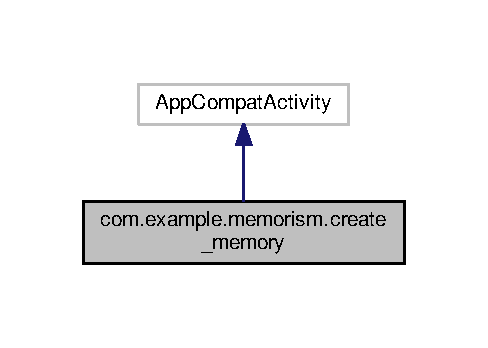
\includegraphics[width=234pt]{d0/dd9/classcom_1_1example_1_1memorism_1_1create__memory__inherit__graph}
\end{center}
\end{figure}


Collaboration diagram for com.\+example.\+memorism.\+create\+\_\+memory\+:\nopagebreak
\begin{figure}[H]
\begin{center}
\leavevmode
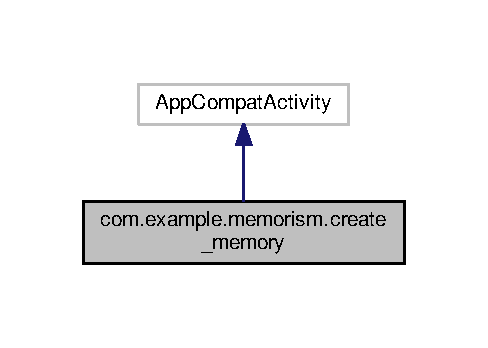
\includegraphics[width=234pt]{d8/d29/classcom_1_1example_1_1memorism_1_1create__memory__coll__graph}
\end{center}
\end{figure}
\subsection*{Static Public Attributes}
\begin{DoxyCompactItemize}
\item 
static String \hyperlink{classcom_1_1example_1_1memorism_1_1create__memory_a6ca3be37a6f7c9d83536809cfbd99dc1}{new\+\_\+id} = U\+U\+I\+D.\+random\+U\+U\+ID().to\+String()
\end{DoxyCompactItemize}
\subsection*{Protected Member Functions}
\begin{DoxyCompactItemize}
\item 
void \hyperlink{classcom_1_1example_1_1memorism_1_1create__memory_ae893508a5c248a70fca50c75c1d7839a}{on\+Create} (Bundle saved\+Instance\+State)
\end{DoxyCompactItemize}


\subsection{Detailed Description}


Definition at line 33 of file create\+\_\+memory.\+java.



\subsection{Member Function Documentation}
\index{com\+::example\+::memorism\+::create\+\_\+memory@{com\+::example\+::memorism\+::create\+\_\+memory}!on\+Create@{on\+Create}}
\index{on\+Create@{on\+Create}!com\+::example\+::memorism\+::create\+\_\+memory@{com\+::example\+::memorism\+::create\+\_\+memory}}
\subsubsection[{\texorpdfstring{on\+Create(\+Bundle saved\+Instance\+State)}{onCreate(Bundle savedInstanceState)}}]{\setlength{\rightskip}{0pt plus 5cm}void com.\+example.\+memorism.\+create\+\_\+memory.\+on\+Create (
\begin{DoxyParamCaption}
\item[{Bundle}]{saved\+Instance\+State}
\end{DoxyParamCaption}
)\hspace{0.3cm}{\ttfamily [protected]}}\hypertarget{classcom_1_1example_1_1memorism_1_1create__memory_ae893508a5c248a70fca50c75c1d7839a}{}\label{classcom_1_1example_1_1memorism_1_1create__memory_ae893508a5c248a70fca50c75c1d7839a}


Definition at line 44 of file create\+\_\+memory.\+java.



\subsection{Member Data Documentation}
\index{com\+::example\+::memorism\+::create\+\_\+memory@{com\+::example\+::memorism\+::create\+\_\+memory}!new\+\_\+id@{new\+\_\+id}}
\index{new\+\_\+id@{new\+\_\+id}!com\+::example\+::memorism\+::create\+\_\+memory@{com\+::example\+::memorism\+::create\+\_\+memory}}
\subsubsection[{\texorpdfstring{new\+\_\+id}{new_id}}]{\setlength{\rightskip}{0pt plus 5cm}String com.\+example.\+memorism.\+create\+\_\+memory.\+new\+\_\+id = U\+U\+I\+D.\+random\+U\+U\+ID().to\+String()\hspace{0.3cm}{\ttfamily [static]}}\hypertarget{classcom_1_1example_1_1memorism_1_1create__memory_a6ca3be37a6f7c9d83536809cfbd99dc1}{}\label{classcom_1_1example_1_1memorism_1_1create__memory_a6ca3be37a6f7c9d83536809cfbd99dc1}


Definition at line 41 of file create\+\_\+memory.\+java.



The documentation for this class was generated from the following file\+:\begin{DoxyCompactItemize}
\item 
/home/farid/\+Android\+Studio\+Projects/\+Memorism/app/src/main/java/com/example/memorism/\hyperlink{create__memory_8java}{create\+\_\+memory.\+java}\end{DoxyCompactItemize}

\input{d8/dc4/classcom_1_1example_1_1memorism_1_1create__trip}
\hypertarget{classcom_1_1example_1_1memorism_1_1memory_1_1_d_b_helper}{}\section{com.\+example.\+memorism.\+memory.\+D\+B\+Helper Class Reference}
\label{classcom_1_1example_1_1memorism_1_1memory_1_1_d_b_helper}\index{com.\+example.\+memorism.\+memory.\+D\+B\+Helper@{com.\+example.\+memorism.\+memory.\+D\+B\+Helper}}


Inheritance diagram for com.\+example.\+memorism.\+memory.\+D\+B\+Helper\+:
\nopagebreak
\begin{figure}[H]
\begin{center}
\leavevmode
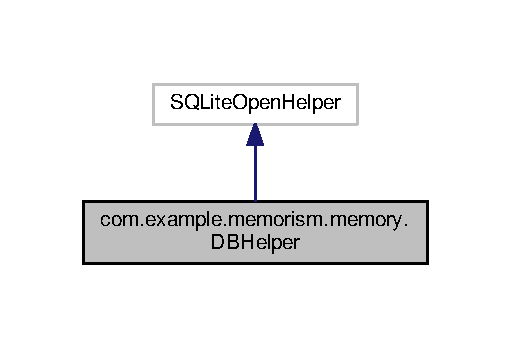
\includegraphics[width=245pt]{d2/d8c/classcom_1_1example_1_1memorism_1_1memory_1_1_d_b_helper__inherit__graph}
\end{center}
\end{figure}


Collaboration diagram for com.\+example.\+memorism.\+memory.\+D\+B\+Helper\+:
\nopagebreak
\begin{figure}[H]
\begin{center}
\leavevmode
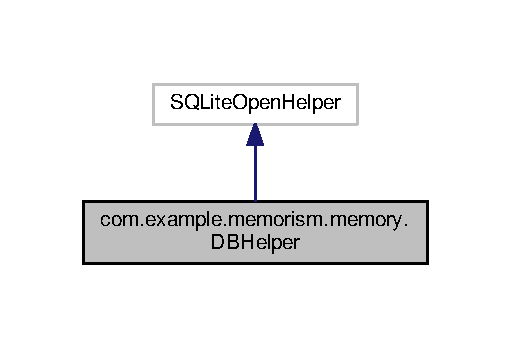
\includegraphics[width=245pt]{d5/d96/classcom_1_1example_1_1memorism_1_1memory_1_1_d_b_helper__coll__graph}
\end{center}
\end{figure}
\subsection*{Public Member Functions}
\begin{DoxyCompactItemize}
\item 
\hyperlink{classcom_1_1example_1_1memorism_1_1memory_1_1_d_b_helper_a1a910311426223624f16314574fc8395}{D\+B\+Helper} (Context context)
\item 
void \hyperlink{classcom_1_1example_1_1memorism_1_1memory_1_1_d_b_helper_af116d080f66582b43bf7cc392862f1cd}{on\+Create} (S\+Q\+Lite\+Database db)
\item 
void \hyperlink{classcom_1_1example_1_1memorism_1_1memory_1_1_d_b_helper_a10e47b5b5978e7f89ec326cf3782c2b0}{on\+Upgrade} (S\+Q\+Lite\+Database db, int old\+Version, int new\+Version)
\item 
void \hyperlink{classcom_1_1example_1_1memorism_1_1memory_1_1_d_b_helper_a5a10d27ab67b8b21fe6a4791138596a2}{reset\+\_\+data\+Base} (S\+Q\+Lite\+Database db)
\item 
boolean \hyperlink{classcom_1_1example_1_1memorism_1_1memory_1_1_d_b_helper_a377fbc795ffd8620bd16276bc373f9e9}{insert\+Memory\+Into\+DB} (Memory\+Content.\+Memory\+Item item)
\item 
Memory\+Content.\+Memory\+Item \hyperlink{classcom_1_1example_1_1memorism_1_1memory_1_1_d_b_helper_ae2b30388cd48178666c0fa93ef9362b6}{get\+Item\+From\+DB} (String date)
\item 
int \hyperlink{classcom_1_1example_1_1memorism_1_1memory_1_1_d_b_helper_ace53414fe54d6caa930a1453ab7d237a}{number\+Of\+Rows} ()
\item 
boolean \hyperlink{classcom_1_1example_1_1memorism_1_1memory_1_1_d_b_helper_aa40fc6dae948e51c155f23695c2af9c6}{update\+Memory} (String date, String new\+Title, String new\+Details, float new\+Latitude, float new\+Longitude)
\item 
Integer \hyperlink{classcom_1_1example_1_1memorism_1_1memory_1_1_d_b_helper_a93e6cb1b1f1bc8d39aeaace04dc92446}{delete\+Memory} (String date)
\item 
void \hyperlink{classcom_1_1example_1_1memorism_1_1memory_1_1_d_b_helper_a82845616a8210bace5188f41aaef1594}{get\+All\+Memory} ()
\end{DoxyCompactItemize}
\subsection*{Static Public Attributes}
\begin{DoxyCompactItemize}
\item 
static final String \hyperlink{classcom_1_1example_1_1memorism_1_1memory_1_1_d_b_helper_a61a19ee13881d07c502373a34687d671}{D\+A\+T\+A\+B\+A\+S\+E\+\_\+\+N\+A\+ME} = \char`\"{}Memorism\+\_\+database.\+db\char`\"{}
\item 
static final String \hyperlink{classcom_1_1example_1_1memorism_1_1memory_1_1_d_b_helper_afb514eee57c4fe21a7c1b7c9c72747a0}{T\+A\+B\+L\+E\+\_\+\+N\+A\+ME} = \char`\"{}memory\+\_\+content\char`\"{}
\item 
static final String \hyperlink{classcom_1_1example_1_1memorism_1_1memory_1_1_d_b_helper_a12593a1ae6e3c03afbc9d108b7c59dff}{C\+O\+L\+U\+M\+N\+\_\+\+ID} = \char`\"{}id\char`\"{}
\item 
static final String \hyperlink{classcom_1_1example_1_1memorism_1_1memory_1_1_d_b_helper_a78ff1252868691cc74b9a20b44849ea5}{C\+O\+L\+U\+M\+N\+\_\+\+D\+A\+TE} = \char`\"{}date\char`\"{}
\item 
static final String \hyperlink{classcom_1_1example_1_1memorism_1_1memory_1_1_d_b_helper_ab96886bfdaf0e3551201f4e03f1e4ad0}{C\+O\+L\+U\+M\+N\+\_\+\+T\+I\+T\+LE} = \char`\"{}title\char`\"{}
\item 
static final String \hyperlink{classcom_1_1example_1_1memorism_1_1memory_1_1_d_b_helper_a43bb30fdefc54ee809ff8517fb0cdbfc}{C\+O\+L\+U\+M\+N\+\_\+\+D\+E\+T\+A\+I\+LS} = \char`\"{}details\char`\"{}
\item 
static final String \hyperlink{classcom_1_1example_1_1memorism_1_1memory_1_1_d_b_helper_a853f90958b6e860ffa3fea8c315b7c26}{C\+O\+L\+U\+M\+N\+\_\+\+L\+O\+N\+G\+I\+T\+U\+DE} = \char`\"{}longitude\char`\"{}
\item 
static final String \hyperlink{classcom_1_1example_1_1memorism_1_1memory_1_1_d_b_helper_aef173dee96dd1d3292ed86bc1394fb37}{C\+O\+L\+U\+M\+N\+\_\+\+L\+A\+T\+I\+T\+U\+DE} = \char`\"{}latitude\char`\"{}
\end{DoxyCompactItemize}


\subsection{Detailed Description}
Created by farid on 27/12/17. 

Definition at line 26 of file D\+B\+Helper.\+java.



\subsection{Constructor \& Destructor Documentation}
\index{com\+::example\+::memorism\+::memory\+::\+D\+B\+Helper@{com\+::example\+::memorism\+::memory\+::\+D\+B\+Helper}!D\+B\+Helper@{D\+B\+Helper}}
\index{D\+B\+Helper@{D\+B\+Helper}!com\+::example\+::memorism\+::memory\+::\+D\+B\+Helper@{com\+::example\+::memorism\+::memory\+::\+D\+B\+Helper}}
\subsubsection[{\texorpdfstring{D\+B\+Helper(\+Context context)}{DBHelper(Context context)}}]{\setlength{\rightskip}{0pt plus 5cm}com.\+example.\+memorism.\+memory.\+D\+B\+Helper.\+D\+B\+Helper (
\begin{DoxyParamCaption}
\item[{Context}]{context}
\end{DoxyParamCaption}
)}\hypertarget{classcom_1_1example_1_1memorism_1_1memory_1_1_d_b_helper_a1a910311426223624f16314574fc8395}{}\label{classcom_1_1example_1_1memorism_1_1memory_1_1_d_b_helper_a1a910311426223624f16314574fc8395}


Definition at line 39 of file D\+B\+Helper.\+java.



\subsection{Member Function Documentation}
\index{com\+::example\+::memorism\+::memory\+::\+D\+B\+Helper@{com\+::example\+::memorism\+::memory\+::\+D\+B\+Helper}!delete\+Memory@{delete\+Memory}}
\index{delete\+Memory@{delete\+Memory}!com\+::example\+::memorism\+::memory\+::\+D\+B\+Helper@{com\+::example\+::memorism\+::memory\+::\+D\+B\+Helper}}
\subsubsection[{\texorpdfstring{delete\+Memory(\+String date)}{deleteMemory(String date)}}]{\setlength{\rightskip}{0pt plus 5cm}Integer com.\+example.\+memorism.\+memory.\+D\+B\+Helper.\+delete\+Memory (
\begin{DoxyParamCaption}
\item[{String}]{date}
\end{DoxyParamCaption}
)}\hypertarget{classcom_1_1example_1_1memorism_1_1memory_1_1_d_b_helper_a93e6cb1b1f1bc8d39aeaace04dc92446}{}\label{classcom_1_1example_1_1memorism_1_1memory_1_1_d_b_helper_a93e6cb1b1f1bc8d39aeaace04dc92446}


Definition at line 128 of file D\+B\+Helper.\+java.

\index{com\+::example\+::memorism\+::memory\+::\+D\+B\+Helper@{com\+::example\+::memorism\+::memory\+::\+D\+B\+Helper}!get\+All\+Memory@{get\+All\+Memory}}
\index{get\+All\+Memory@{get\+All\+Memory}!com\+::example\+::memorism\+::memory\+::\+D\+B\+Helper@{com\+::example\+::memorism\+::memory\+::\+D\+B\+Helper}}
\subsubsection[{\texorpdfstring{get\+All\+Memory()}{getAllMemory()}}]{\setlength{\rightskip}{0pt plus 5cm}void com.\+example.\+memorism.\+memory.\+D\+B\+Helper.\+get\+All\+Memory (
\begin{DoxyParamCaption}
{}
\end{DoxyParamCaption}
)}\hypertarget{classcom_1_1example_1_1memorism_1_1memory_1_1_d_b_helper_a82845616a8210bace5188f41aaef1594}{}\label{classcom_1_1example_1_1memorism_1_1memory_1_1_d_b_helper_a82845616a8210bace5188f41aaef1594}


Definition at line 135 of file D\+B\+Helper.\+java.

\index{com\+::example\+::memorism\+::memory\+::\+D\+B\+Helper@{com\+::example\+::memorism\+::memory\+::\+D\+B\+Helper}!get\+Item\+From\+DB@{get\+Item\+From\+DB}}
\index{get\+Item\+From\+DB@{get\+Item\+From\+DB}!com\+::example\+::memorism\+::memory\+::\+D\+B\+Helper@{com\+::example\+::memorism\+::memory\+::\+D\+B\+Helper}}
\subsubsection[{\texorpdfstring{get\+Item\+From\+D\+B(\+String date)}{getItemFromDB(String date)}}]{\setlength{\rightskip}{0pt plus 5cm}Memory\+Content.\+Memory\+Item com.\+example.\+memorism.\+memory.\+D\+B\+Helper.\+get\+Item\+From\+DB (
\begin{DoxyParamCaption}
\item[{String}]{date}
\end{DoxyParamCaption}
)}\hypertarget{classcom_1_1example_1_1memorism_1_1memory_1_1_d_b_helper_ae2b30388cd48178666c0fa93ef9362b6}{}\label{classcom_1_1example_1_1memorism_1_1memory_1_1_d_b_helper_ae2b30388cd48178666c0fa93ef9362b6}


Definition at line 98 of file D\+B\+Helper.\+java.

\index{com\+::example\+::memorism\+::memory\+::\+D\+B\+Helper@{com\+::example\+::memorism\+::memory\+::\+D\+B\+Helper}!insert\+Memory\+Into\+DB@{insert\+Memory\+Into\+DB}}
\index{insert\+Memory\+Into\+DB@{insert\+Memory\+Into\+DB}!com\+::example\+::memorism\+::memory\+::\+D\+B\+Helper@{com\+::example\+::memorism\+::memory\+::\+D\+B\+Helper}}
\subsubsection[{\texorpdfstring{insert\+Memory\+Into\+D\+B(\+Memory\+Content.\+Memory\+Item item)}{insertMemoryIntoDB(MemoryContent.MemoryItem item)}}]{\setlength{\rightskip}{0pt plus 5cm}boolean com.\+example.\+memorism.\+memory.\+D\+B\+Helper.\+insert\+Memory\+Into\+DB (
\begin{DoxyParamCaption}
\item[{Memory\+Content.\+Memory\+Item}]{item}
\end{DoxyParamCaption}
)}\hypertarget{classcom_1_1example_1_1memorism_1_1memory_1_1_d_b_helper_a377fbc795ffd8620bd16276bc373f9e9}{}\label{classcom_1_1example_1_1memorism_1_1memory_1_1_d_b_helper_a377fbc795ffd8620bd16276bc373f9e9}


Definition at line 86 of file D\+B\+Helper.\+java.

\index{com\+::example\+::memorism\+::memory\+::\+D\+B\+Helper@{com\+::example\+::memorism\+::memory\+::\+D\+B\+Helper}!number\+Of\+Rows@{number\+Of\+Rows}}
\index{number\+Of\+Rows@{number\+Of\+Rows}!com\+::example\+::memorism\+::memory\+::\+D\+B\+Helper@{com\+::example\+::memorism\+::memory\+::\+D\+B\+Helper}}
\subsubsection[{\texorpdfstring{number\+Of\+Rows()}{numberOfRows()}}]{\setlength{\rightskip}{0pt plus 5cm}int com.\+example.\+memorism.\+memory.\+D\+B\+Helper.\+number\+Of\+Rows (
\begin{DoxyParamCaption}
{}
\end{DoxyParamCaption}
)}\hypertarget{classcom_1_1example_1_1memorism_1_1memory_1_1_d_b_helper_ace53414fe54d6caa930a1453ab7d237a}{}\label{classcom_1_1example_1_1memorism_1_1memory_1_1_d_b_helper_ace53414fe54d6caa930a1453ab7d237a}


Definition at line 110 of file D\+B\+Helper.\+java.

\index{com\+::example\+::memorism\+::memory\+::\+D\+B\+Helper@{com\+::example\+::memorism\+::memory\+::\+D\+B\+Helper}!on\+Create@{on\+Create}}
\index{on\+Create@{on\+Create}!com\+::example\+::memorism\+::memory\+::\+D\+B\+Helper@{com\+::example\+::memorism\+::memory\+::\+D\+B\+Helper}}
\subsubsection[{\texorpdfstring{on\+Create(\+S\+Q\+Lite\+Database db)}{onCreate(SQLiteDatabase db)}}]{\setlength{\rightskip}{0pt plus 5cm}void com.\+example.\+memorism.\+memory.\+D\+B\+Helper.\+on\+Create (
\begin{DoxyParamCaption}
\item[{S\+Q\+Lite\+Database}]{db}
\end{DoxyParamCaption}
)}\hypertarget{classcom_1_1example_1_1memorism_1_1memory_1_1_d_b_helper_af116d080f66582b43bf7cc392862f1cd}{}\label{classcom_1_1example_1_1memorism_1_1memory_1_1_d_b_helper_af116d080f66582b43bf7cc392862f1cd}


Definition at line 45 of file D\+B\+Helper.\+java.

\index{com\+::example\+::memorism\+::memory\+::\+D\+B\+Helper@{com\+::example\+::memorism\+::memory\+::\+D\+B\+Helper}!on\+Upgrade@{on\+Upgrade}}
\index{on\+Upgrade@{on\+Upgrade}!com\+::example\+::memorism\+::memory\+::\+D\+B\+Helper@{com\+::example\+::memorism\+::memory\+::\+D\+B\+Helper}}
\subsubsection[{\texorpdfstring{on\+Upgrade(\+S\+Q\+Lite\+Database db, int old\+Version, int new\+Version)}{onUpgrade(SQLiteDatabase db, int oldVersion, int newVersion)}}]{\setlength{\rightskip}{0pt plus 5cm}void com.\+example.\+memorism.\+memory.\+D\+B\+Helper.\+on\+Upgrade (
\begin{DoxyParamCaption}
\item[{S\+Q\+Lite\+Database}]{db, }
\item[{int}]{old\+Version, }
\item[{int}]{new\+Version}
\end{DoxyParamCaption}
)}\hypertarget{classcom_1_1example_1_1memorism_1_1memory_1_1_d_b_helper_a10e47b5b5978e7f89ec326cf3782c2b0}{}\label{classcom_1_1example_1_1memorism_1_1memory_1_1_d_b_helper_a10e47b5b5978e7f89ec326cf3782c2b0}


Definition at line 74 of file D\+B\+Helper.\+java.

\index{com\+::example\+::memorism\+::memory\+::\+D\+B\+Helper@{com\+::example\+::memorism\+::memory\+::\+D\+B\+Helper}!reset\+\_\+data\+Base@{reset\+\_\+data\+Base}}
\index{reset\+\_\+data\+Base@{reset\+\_\+data\+Base}!com\+::example\+::memorism\+::memory\+::\+D\+B\+Helper@{com\+::example\+::memorism\+::memory\+::\+D\+B\+Helper}}
\subsubsection[{\texorpdfstring{reset\+\_\+data\+Base(\+S\+Q\+Lite\+Database db)}{reset_dataBase(SQLiteDatabase db)}}]{\setlength{\rightskip}{0pt plus 5cm}void com.\+example.\+memorism.\+memory.\+D\+B\+Helper.\+reset\+\_\+data\+Base (
\begin{DoxyParamCaption}
\item[{S\+Q\+Lite\+Database}]{db}
\end{DoxyParamCaption}
)}\hypertarget{classcom_1_1example_1_1memorism_1_1memory_1_1_d_b_helper_a5a10d27ab67b8b21fe6a4791138596a2}{}\label{classcom_1_1example_1_1memorism_1_1memory_1_1_d_b_helper_a5a10d27ab67b8b21fe6a4791138596a2}


Definition at line 80 of file D\+B\+Helper.\+java.

\index{com\+::example\+::memorism\+::memory\+::\+D\+B\+Helper@{com\+::example\+::memorism\+::memory\+::\+D\+B\+Helper}!update\+Memory@{update\+Memory}}
\index{update\+Memory@{update\+Memory}!com\+::example\+::memorism\+::memory\+::\+D\+B\+Helper@{com\+::example\+::memorism\+::memory\+::\+D\+B\+Helper}}
\subsubsection[{\texorpdfstring{update\+Memory(\+String date, String new\+Title, String new\+Details, float new\+Latitude, float new\+Longitude)}{updateMemory(String date, String newTitle, String newDetails, float newLatitude, float newLongitude)}}]{\setlength{\rightskip}{0pt plus 5cm}boolean com.\+example.\+memorism.\+memory.\+D\+B\+Helper.\+update\+Memory (
\begin{DoxyParamCaption}
\item[{String}]{date, }
\item[{String}]{new\+Title, }
\item[{String}]{new\+Details, }
\item[{float}]{new\+Latitude, }
\item[{float}]{new\+Longitude}
\end{DoxyParamCaption}
)}\hypertarget{classcom_1_1example_1_1memorism_1_1memory_1_1_d_b_helper_aa40fc6dae948e51c155f23695c2af9c6}{}\label{classcom_1_1example_1_1memorism_1_1memory_1_1_d_b_helper_aa40fc6dae948e51c155f23695c2af9c6}


Definition at line 116 of file D\+B\+Helper.\+java.



\subsection{Member Data Documentation}
\index{com\+::example\+::memorism\+::memory\+::\+D\+B\+Helper@{com\+::example\+::memorism\+::memory\+::\+D\+B\+Helper}!C\+O\+L\+U\+M\+N\+\_\+\+D\+A\+TE@{C\+O\+L\+U\+M\+N\+\_\+\+D\+A\+TE}}
\index{C\+O\+L\+U\+M\+N\+\_\+\+D\+A\+TE@{C\+O\+L\+U\+M\+N\+\_\+\+D\+A\+TE}!com\+::example\+::memorism\+::memory\+::\+D\+B\+Helper@{com\+::example\+::memorism\+::memory\+::\+D\+B\+Helper}}
\subsubsection[{\texorpdfstring{C\+O\+L\+U\+M\+N\+\_\+\+D\+A\+TE}{COLUMN_DATE}}]{\setlength{\rightskip}{0pt plus 5cm}final String com.\+example.\+memorism.\+memory.\+D\+B\+Helper.\+C\+O\+L\+U\+M\+N\+\_\+\+D\+A\+TE = \char`\"{}date\char`\"{}\hspace{0.3cm}{\ttfamily [static]}}\hypertarget{classcom_1_1example_1_1memorism_1_1memory_1_1_d_b_helper_a78ff1252868691cc74b9a20b44849ea5}{}\label{classcom_1_1example_1_1memorism_1_1memory_1_1_d_b_helper_a78ff1252868691cc74b9a20b44849ea5}


Definition at line 33 of file D\+B\+Helper.\+java.

\index{com\+::example\+::memorism\+::memory\+::\+D\+B\+Helper@{com\+::example\+::memorism\+::memory\+::\+D\+B\+Helper}!C\+O\+L\+U\+M\+N\+\_\+\+D\+E\+T\+A\+I\+LS@{C\+O\+L\+U\+M\+N\+\_\+\+D\+E\+T\+A\+I\+LS}}
\index{C\+O\+L\+U\+M\+N\+\_\+\+D\+E\+T\+A\+I\+LS@{C\+O\+L\+U\+M\+N\+\_\+\+D\+E\+T\+A\+I\+LS}!com\+::example\+::memorism\+::memory\+::\+D\+B\+Helper@{com\+::example\+::memorism\+::memory\+::\+D\+B\+Helper}}
\subsubsection[{\texorpdfstring{C\+O\+L\+U\+M\+N\+\_\+\+D\+E\+T\+A\+I\+LS}{COLUMN_DETAILS}}]{\setlength{\rightskip}{0pt plus 5cm}final String com.\+example.\+memorism.\+memory.\+D\+B\+Helper.\+C\+O\+L\+U\+M\+N\+\_\+\+D\+E\+T\+A\+I\+LS = \char`\"{}details\char`\"{}\hspace{0.3cm}{\ttfamily [static]}}\hypertarget{classcom_1_1example_1_1memorism_1_1memory_1_1_d_b_helper_a43bb30fdefc54ee809ff8517fb0cdbfc}{}\label{classcom_1_1example_1_1memorism_1_1memory_1_1_d_b_helper_a43bb30fdefc54ee809ff8517fb0cdbfc}


Definition at line 35 of file D\+B\+Helper.\+java.

\index{com\+::example\+::memorism\+::memory\+::\+D\+B\+Helper@{com\+::example\+::memorism\+::memory\+::\+D\+B\+Helper}!C\+O\+L\+U\+M\+N\+\_\+\+ID@{C\+O\+L\+U\+M\+N\+\_\+\+ID}}
\index{C\+O\+L\+U\+M\+N\+\_\+\+ID@{C\+O\+L\+U\+M\+N\+\_\+\+ID}!com\+::example\+::memorism\+::memory\+::\+D\+B\+Helper@{com\+::example\+::memorism\+::memory\+::\+D\+B\+Helper}}
\subsubsection[{\texorpdfstring{C\+O\+L\+U\+M\+N\+\_\+\+ID}{COLUMN_ID}}]{\setlength{\rightskip}{0pt plus 5cm}final String com.\+example.\+memorism.\+memory.\+D\+B\+Helper.\+C\+O\+L\+U\+M\+N\+\_\+\+ID = \char`\"{}id\char`\"{}\hspace{0.3cm}{\ttfamily [static]}}\hypertarget{classcom_1_1example_1_1memorism_1_1memory_1_1_d_b_helper_a12593a1ae6e3c03afbc9d108b7c59dff}{}\label{classcom_1_1example_1_1memorism_1_1memory_1_1_d_b_helper_a12593a1ae6e3c03afbc9d108b7c59dff}


Definition at line 32 of file D\+B\+Helper.\+java.

\index{com\+::example\+::memorism\+::memory\+::\+D\+B\+Helper@{com\+::example\+::memorism\+::memory\+::\+D\+B\+Helper}!C\+O\+L\+U\+M\+N\+\_\+\+L\+A\+T\+I\+T\+U\+DE@{C\+O\+L\+U\+M\+N\+\_\+\+L\+A\+T\+I\+T\+U\+DE}}
\index{C\+O\+L\+U\+M\+N\+\_\+\+L\+A\+T\+I\+T\+U\+DE@{C\+O\+L\+U\+M\+N\+\_\+\+L\+A\+T\+I\+T\+U\+DE}!com\+::example\+::memorism\+::memory\+::\+D\+B\+Helper@{com\+::example\+::memorism\+::memory\+::\+D\+B\+Helper}}
\subsubsection[{\texorpdfstring{C\+O\+L\+U\+M\+N\+\_\+\+L\+A\+T\+I\+T\+U\+DE}{COLUMN_LATITUDE}}]{\setlength{\rightskip}{0pt plus 5cm}final String com.\+example.\+memorism.\+memory.\+D\+B\+Helper.\+C\+O\+L\+U\+M\+N\+\_\+\+L\+A\+T\+I\+T\+U\+DE = \char`\"{}latitude\char`\"{}\hspace{0.3cm}{\ttfamily [static]}}\hypertarget{classcom_1_1example_1_1memorism_1_1memory_1_1_d_b_helper_aef173dee96dd1d3292ed86bc1394fb37}{}\label{classcom_1_1example_1_1memorism_1_1memory_1_1_d_b_helper_aef173dee96dd1d3292ed86bc1394fb37}


Definition at line 37 of file D\+B\+Helper.\+java.

\index{com\+::example\+::memorism\+::memory\+::\+D\+B\+Helper@{com\+::example\+::memorism\+::memory\+::\+D\+B\+Helper}!C\+O\+L\+U\+M\+N\+\_\+\+L\+O\+N\+G\+I\+T\+U\+DE@{C\+O\+L\+U\+M\+N\+\_\+\+L\+O\+N\+G\+I\+T\+U\+DE}}
\index{C\+O\+L\+U\+M\+N\+\_\+\+L\+O\+N\+G\+I\+T\+U\+DE@{C\+O\+L\+U\+M\+N\+\_\+\+L\+O\+N\+G\+I\+T\+U\+DE}!com\+::example\+::memorism\+::memory\+::\+D\+B\+Helper@{com\+::example\+::memorism\+::memory\+::\+D\+B\+Helper}}
\subsubsection[{\texorpdfstring{C\+O\+L\+U\+M\+N\+\_\+\+L\+O\+N\+G\+I\+T\+U\+DE}{COLUMN_LONGITUDE}}]{\setlength{\rightskip}{0pt plus 5cm}final String com.\+example.\+memorism.\+memory.\+D\+B\+Helper.\+C\+O\+L\+U\+M\+N\+\_\+\+L\+O\+N\+G\+I\+T\+U\+DE = \char`\"{}longitude\char`\"{}\hspace{0.3cm}{\ttfamily [static]}}\hypertarget{classcom_1_1example_1_1memorism_1_1memory_1_1_d_b_helper_a853f90958b6e860ffa3fea8c315b7c26}{}\label{classcom_1_1example_1_1memorism_1_1memory_1_1_d_b_helper_a853f90958b6e860ffa3fea8c315b7c26}


Definition at line 36 of file D\+B\+Helper.\+java.

\index{com\+::example\+::memorism\+::memory\+::\+D\+B\+Helper@{com\+::example\+::memorism\+::memory\+::\+D\+B\+Helper}!C\+O\+L\+U\+M\+N\+\_\+\+T\+I\+T\+LE@{C\+O\+L\+U\+M\+N\+\_\+\+T\+I\+T\+LE}}
\index{C\+O\+L\+U\+M\+N\+\_\+\+T\+I\+T\+LE@{C\+O\+L\+U\+M\+N\+\_\+\+T\+I\+T\+LE}!com\+::example\+::memorism\+::memory\+::\+D\+B\+Helper@{com\+::example\+::memorism\+::memory\+::\+D\+B\+Helper}}
\subsubsection[{\texorpdfstring{C\+O\+L\+U\+M\+N\+\_\+\+T\+I\+T\+LE}{COLUMN_TITLE}}]{\setlength{\rightskip}{0pt plus 5cm}final String com.\+example.\+memorism.\+memory.\+D\+B\+Helper.\+C\+O\+L\+U\+M\+N\+\_\+\+T\+I\+T\+LE = \char`\"{}title\char`\"{}\hspace{0.3cm}{\ttfamily [static]}}\hypertarget{classcom_1_1example_1_1memorism_1_1memory_1_1_d_b_helper_ab96886bfdaf0e3551201f4e03f1e4ad0}{}\label{classcom_1_1example_1_1memorism_1_1memory_1_1_d_b_helper_ab96886bfdaf0e3551201f4e03f1e4ad0}


Definition at line 34 of file D\+B\+Helper.\+java.

\index{com\+::example\+::memorism\+::memory\+::\+D\+B\+Helper@{com\+::example\+::memorism\+::memory\+::\+D\+B\+Helper}!D\+A\+T\+A\+B\+A\+S\+E\+\_\+\+N\+A\+ME@{D\+A\+T\+A\+B\+A\+S\+E\+\_\+\+N\+A\+ME}}
\index{D\+A\+T\+A\+B\+A\+S\+E\+\_\+\+N\+A\+ME@{D\+A\+T\+A\+B\+A\+S\+E\+\_\+\+N\+A\+ME}!com\+::example\+::memorism\+::memory\+::\+D\+B\+Helper@{com\+::example\+::memorism\+::memory\+::\+D\+B\+Helper}}
\subsubsection[{\texorpdfstring{D\+A\+T\+A\+B\+A\+S\+E\+\_\+\+N\+A\+ME}{DATABASE_NAME}}]{\setlength{\rightskip}{0pt plus 5cm}final String com.\+example.\+memorism.\+memory.\+D\+B\+Helper.\+D\+A\+T\+A\+B\+A\+S\+E\+\_\+\+N\+A\+ME = \char`\"{}Memorism\+\_\+database.\+db\char`\"{}\hspace{0.3cm}{\ttfamily [static]}}\hypertarget{classcom_1_1example_1_1memorism_1_1memory_1_1_d_b_helper_a61a19ee13881d07c502373a34687d671}{}\label{classcom_1_1example_1_1memorism_1_1memory_1_1_d_b_helper_a61a19ee13881d07c502373a34687d671}


Definition at line 30 of file D\+B\+Helper.\+java.

\index{com\+::example\+::memorism\+::memory\+::\+D\+B\+Helper@{com\+::example\+::memorism\+::memory\+::\+D\+B\+Helper}!T\+A\+B\+L\+E\+\_\+\+N\+A\+ME@{T\+A\+B\+L\+E\+\_\+\+N\+A\+ME}}
\index{T\+A\+B\+L\+E\+\_\+\+N\+A\+ME@{T\+A\+B\+L\+E\+\_\+\+N\+A\+ME}!com\+::example\+::memorism\+::memory\+::\+D\+B\+Helper@{com\+::example\+::memorism\+::memory\+::\+D\+B\+Helper}}
\subsubsection[{\texorpdfstring{T\+A\+B\+L\+E\+\_\+\+N\+A\+ME}{TABLE_NAME}}]{\setlength{\rightskip}{0pt plus 5cm}final String com.\+example.\+memorism.\+memory.\+D\+B\+Helper.\+T\+A\+B\+L\+E\+\_\+\+N\+A\+ME = \char`\"{}memory\+\_\+content\char`\"{}\hspace{0.3cm}{\ttfamily [static]}}\hypertarget{classcom_1_1example_1_1memorism_1_1memory_1_1_d_b_helper_afb514eee57c4fe21a7c1b7c9c72747a0}{}\label{classcom_1_1example_1_1memorism_1_1memory_1_1_d_b_helper_afb514eee57c4fe21a7c1b7c9c72747a0}


Definition at line 31 of file D\+B\+Helper.\+java.



The documentation for this class was generated from the following file\+:\begin{DoxyCompactItemize}
\item 
/home/farid/\+Android\+Studio\+Projects/\+Memorism/app/src/main/java/com/example/memorism/memory/\hyperlink{_d_b_helper_8java}{D\+B\+Helper.\+java}\end{DoxyCompactItemize}

\hypertarget{classcom_1_1example_1_1memorism_1_1_g_p_stracker}{}\section{com.\+example.\+memorism.\+G\+P\+Stracker Class Reference}
\label{classcom_1_1example_1_1memorism_1_1_g_p_stracker}\index{com.\+example.\+memorism.\+G\+P\+Stracker@{com.\+example.\+memorism.\+G\+P\+Stracker}}


Inheritance diagram for com.\+example.\+memorism.\+G\+P\+Stracker\+:
\nopagebreak
\begin{figure}[H]
\begin{center}
\leavevmode
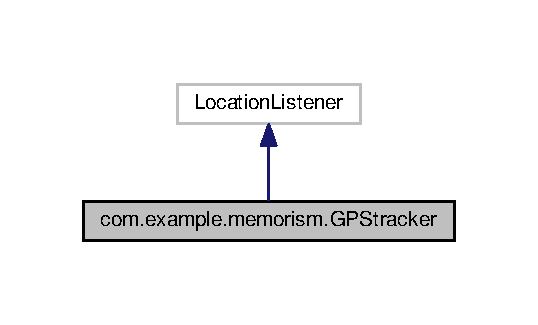
\includegraphics[width=258pt]{dc/d42/classcom_1_1example_1_1memorism_1_1_g_p_stracker__inherit__graph}
\end{center}
\end{figure}


Collaboration diagram for com.\+example.\+memorism.\+G\+P\+Stracker\+:
\nopagebreak
\begin{figure}[H]
\begin{center}
\leavevmode
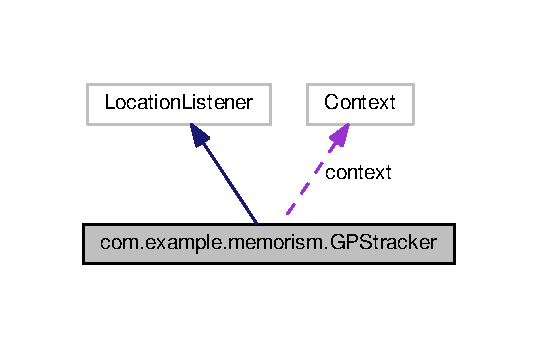
\includegraphics[width=258pt]{de/df9/classcom_1_1example_1_1memorism_1_1_g_p_stracker__coll__graph}
\end{center}
\end{figure}
\subsection*{Public Member Functions}
\begin{DoxyCompactItemize}
\item 
\hyperlink{classcom_1_1example_1_1memorism_1_1_g_p_stracker_a9631c4882dc9818c92ba9cadd07883a9}{G\+P\+Stracker} (Context c)
\item 
Location \hyperlink{classcom_1_1example_1_1memorism_1_1_g_p_stracker_a1cf48f5065e34c9601f87aa13802b27b}{get\+Location} ()
\item 
void \hyperlink{classcom_1_1example_1_1memorism_1_1_g_p_stracker_ac9fd5b1f5b024c373724f723963316a7}{on\+Location\+Changed} (Location location)
\item 
void \hyperlink{classcom_1_1example_1_1memorism_1_1_g_p_stracker_a7ed31a4aaaadc30b931872c0fa6547a8}{on\+Status\+Changed} (String provider, int status, Bundle extras)
\item 
void \hyperlink{classcom_1_1example_1_1memorism_1_1_g_p_stracker_a32e9b0f373ad99fa6dc0f23aa11c820e}{on\+Provider\+Enabled} (String provider)
\item 
void \hyperlink{classcom_1_1example_1_1memorism_1_1_g_p_stracker_a1a18e037edef5966146afb3e5d7b648a}{on\+Provider\+Disabled} (String provider)
\end{DoxyCompactItemize}


\subsection{Detailed Description}
Created by farid on 27/12/17. 

Definition at line 17 of file G\+P\+Stracker.\+java.



\subsection{Constructor \& Destructor Documentation}
\index{com\+::example\+::memorism\+::\+G\+P\+Stracker@{com\+::example\+::memorism\+::\+G\+P\+Stracker}!G\+P\+Stracker@{G\+P\+Stracker}}
\index{G\+P\+Stracker@{G\+P\+Stracker}!com\+::example\+::memorism\+::\+G\+P\+Stracker@{com\+::example\+::memorism\+::\+G\+P\+Stracker}}
\subsubsection[{\texorpdfstring{G\+P\+Stracker(\+Context c)}{GPStracker(Context c)}}]{\setlength{\rightskip}{0pt plus 5cm}com.\+example.\+memorism.\+G\+P\+Stracker.\+G\+P\+Stracker (
\begin{DoxyParamCaption}
\item[{Context}]{c}
\end{DoxyParamCaption}
)}\hypertarget{classcom_1_1example_1_1memorism_1_1_g_p_stracker_a9631c4882dc9818c92ba9cadd07883a9}{}\label{classcom_1_1example_1_1memorism_1_1_g_p_stracker_a9631c4882dc9818c92ba9cadd07883a9}


Definition at line 21 of file G\+P\+Stracker.\+java.



\subsection{Member Function Documentation}
\index{com\+::example\+::memorism\+::\+G\+P\+Stracker@{com\+::example\+::memorism\+::\+G\+P\+Stracker}!get\+Location@{get\+Location}}
\index{get\+Location@{get\+Location}!com\+::example\+::memorism\+::\+G\+P\+Stracker@{com\+::example\+::memorism\+::\+G\+P\+Stracker}}
\subsubsection[{\texorpdfstring{get\+Location()}{getLocation()}}]{\setlength{\rightskip}{0pt plus 5cm}Location com.\+example.\+memorism.\+G\+P\+Stracker.\+get\+Location (
\begin{DoxyParamCaption}
{}
\end{DoxyParamCaption}
)}\hypertarget{classcom_1_1example_1_1memorism_1_1_g_p_stracker_a1cf48f5065e34c9601f87aa13802b27b}{}\label{classcom_1_1example_1_1memorism_1_1_g_p_stracker_a1cf48f5065e34c9601f87aa13802b27b}


Definition at line 25 of file G\+P\+Stracker.\+java.

\index{com\+::example\+::memorism\+::\+G\+P\+Stracker@{com\+::example\+::memorism\+::\+G\+P\+Stracker}!on\+Location\+Changed@{on\+Location\+Changed}}
\index{on\+Location\+Changed@{on\+Location\+Changed}!com\+::example\+::memorism\+::\+G\+P\+Stracker@{com\+::example\+::memorism\+::\+G\+P\+Stracker}}
\subsubsection[{\texorpdfstring{on\+Location\+Changed(\+Location location)}{onLocationChanged(Location location)}}]{\setlength{\rightskip}{0pt plus 5cm}void com.\+example.\+memorism.\+G\+P\+Stracker.\+on\+Location\+Changed (
\begin{DoxyParamCaption}
\item[{Location}]{location}
\end{DoxyParamCaption}
)}\hypertarget{classcom_1_1example_1_1memorism_1_1_g_p_stracker_ac9fd5b1f5b024c373724f723963316a7}{}\label{classcom_1_1example_1_1memorism_1_1_g_p_stracker_ac9fd5b1f5b024c373724f723963316a7}


Definition at line 47 of file G\+P\+Stracker.\+java.

\index{com\+::example\+::memorism\+::\+G\+P\+Stracker@{com\+::example\+::memorism\+::\+G\+P\+Stracker}!on\+Provider\+Disabled@{on\+Provider\+Disabled}}
\index{on\+Provider\+Disabled@{on\+Provider\+Disabled}!com\+::example\+::memorism\+::\+G\+P\+Stracker@{com\+::example\+::memorism\+::\+G\+P\+Stracker}}
\subsubsection[{\texorpdfstring{on\+Provider\+Disabled(\+String provider)}{onProviderDisabled(String provider)}}]{\setlength{\rightskip}{0pt plus 5cm}void com.\+example.\+memorism.\+G\+P\+Stracker.\+on\+Provider\+Disabled (
\begin{DoxyParamCaption}
\item[{String}]{provider}
\end{DoxyParamCaption}
)}\hypertarget{classcom_1_1example_1_1memorism_1_1_g_p_stracker_a1a18e037edef5966146afb3e5d7b648a}{}\label{classcom_1_1example_1_1memorism_1_1_g_p_stracker_a1a18e037edef5966146afb3e5d7b648a}


Definition at line 62 of file G\+P\+Stracker.\+java.

\index{com\+::example\+::memorism\+::\+G\+P\+Stracker@{com\+::example\+::memorism\+::\+G\+P\+Stracker}!on\+Provider\+Enabled@{on\+Provider\+Enabled}}
\index{on\+Provider\+Enabled@{on\+Provider\+Enabled}!com\+::example\+::memorism\+::\+G\+P\+Stracker@{com\+::example\+::memorism\+::\+G\+P\+Stracker}}
\subsubsection[{\texorpdfstring{on\+Provider\+Enabled(\+String provider)}{onProviderEnabled(String provider)}}]{\setlength{\rightskip}{0pt plus 5cm}void com.\+example.\+memorism.\+G\+P\+Stracker.\+on\+Provider\+Enabled (
\begin{DoxyParamCaption}
\item[{String}]{provider}
\end{DoxyParamCaption}
)}\hypertarget{classcom_1_1example_1_1memorism_1_1_g_p_stracker_a32e9b0f373ad99fa6dc0f23aa11c820e}{}\label{classcom_1_1example_1_1memorism_1_1_g_p_stracker_a32e9b0f373ad99fa6dc0f23aa11c820e}


Definition at line 57 of file G\+P\+Stracker.\+java.

\index{com\+::example\+::memorism\+::\+G\+P\+Stracker@{com\+::example\+::memorism\+::\+G\+P\+Stracker}!on\+Status\+Changed@{on\+Status\+Changed}}
\index{on\+Status\+Changed@{on\+Status\+Changed}!com\+::example\+::memorism\+::\+G\+P\+Stracker@{com\+::example\+::memorism\+::\+G\+P\+Stracker}}
\subsubsection[{\texorpdfstring{on\+Status\+Changed(\+String provider, int status, Bundle extras)}{onStatusChanged(String provider, int status, Bundle extras)}}]{\setlength{\rightskip}{0pt plus 5cm}void com.\+example.\+memorism.\+G\+P\+Stracker.\+on\+Status\+Changed (
\begin{DoxyParamCaption}
\item[{String}]{provider, }
\item[{int}]{status, }
\item[{Bundle}]{extras}
\end{DoxyParamCaption}
)}\hypertarget{classcom_1_1example_1_1memorism_1_1_g_p_stracker_a7ed31a4aaaadc30b931872c0fa6547a8}{}\label{classcom_1_1example_1_1memorism_1_1_g_p_stracker_a7ed31a4aaaadc30b931872c0fa6547a8}


Definition at line 52 of file G\+P\+Stracker.\+java.



The documentation for this class was generated from the following file\+:\begin{DoxyCompactItemize}
\item 
/home/farid/\+Android\+Studio\+Projects/\+Memorism/app/src/main/java/com/example/memorism/\hyperlink{_g_p_stracker_8java}{G\+P\+Stracker.\+java}\end{DoxyCompactItemize}

\hypertarget{classcom_1_1example_1_1memorism_1_1_item_detail_activity}{}\section{com.\+example.\+memorism.\+Item\+Detail\+Activity Class Reference}
\label{classcom_1_1example_1_1memorism_1_1_item_detail_activity}\index{com.\+example.\+memorism.\+Item\+Detail\+Activity@{com.\+example.\+memorism.\+Item\+Detail\+Activity}}


Inheritance diagram for com.\+example.\+memorism.\+Item\+Detail\+Activity\+:
\nopagebreak
\begin{figure}[H]
\begin{center}
\leavevmode
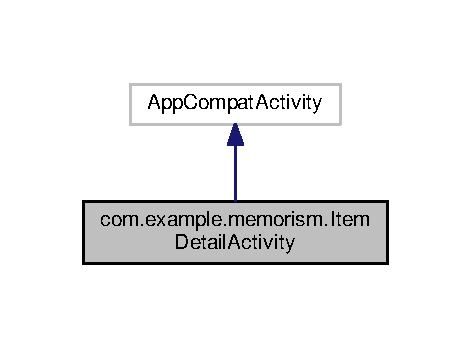
\includegraphics[width=226pt]{d6/d8a/classcom_1_1example_1_1memorism_1_1_item_detail_activity__inherit__graph}
\end{center}
\end{figure}


Collaboration diagram for com.\+example.\+memorism.\+Item\+Detail\+Activity\+:
\nopagebreak
\begin{figure}[H]
\begin{center}
\leavevmode
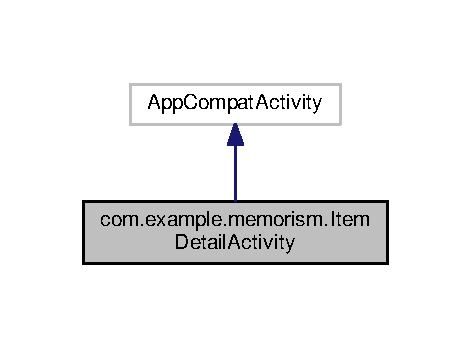
\includegraphics[width=226pt]{d8/deb/classcom_1_1example_1_1memorism_1_1_item_detail_activity__coll__graph}
\end{center}
\end{figure}
\subsection*{Public Member Functions}
\begin{DoxyCompactItemize}
\item 
boolean \hyperlink{classcom_1_1example_1_1memorism_1_1_item_detail_activity_af86a22f6772eb4109179456eeb1ecd4e}{on\+Options\+Item\+Selected} (Menu\+Item item)
\end{DoxyCompactItemize}
\subsection*{Protected Member Functions}
\begin{DoxyCompactItemize}
\item 
void \hyperlink{classcom_1_1example_1_1memorism_1_1_item_detail_activity_aad6ee0faf03666f8b3c67b6a0b8be479}{on\+Create} (Bundle saved\+Instance\+State)
\end{DoxyCompactItemize}


\subsection{Detailed Description}
An activity representing a single Item detail screen. This activity is only used on narrow width devices. On tablet-\/size devices, item details are presented side-\/by-\/side with a list of items in a \hyperlink{classcom_1_1example_1_1memorism_1_1_item_list_activity}{Item\+List\+Activity}. 

Definition at line 20 of file Item\+Detail\+Activity.\+java.



\subsection{Member Function Documentation}
\index{com\+::example\+::memorism\+::\+Item\+Detail\+Activity@{com\+::example\+::memorism\+::\+Item\+Detail\+Activity}!on\+Create@{on\+Create}}
\index{on\+Create@{on\+Create}!com\+::example\+::memorism\+::\+Item\+Detail\+Activity@{com\+::example\+::memorism\+::\+Item\+Detail\+Activity}}
\subsubsection[{\texorpdfstring{on\+Create(\+Bundle saved\+Instance\+State)}{onCreate(Bundle savedInstanceState)}}]{\setlength{\rightskip}{0pt plus 5cm}void com.\+example.\+memorism.\+Item\+Detail\+Activity.\+on\+Create (
\begin{DoxyParamCaption}
\item[{Bundle}]{saved\+Instance\+State}
\end{DoxyParamCaption}
)\hspace{0.3cm}{\ttfamily [protected]}}\hypertarget{classcom_1_1example_1_1memorism_1_1_item_detail_activity_aad6ee0faf03666f8b3c67b6a0b8be479}{}\label{classcom_1_1example_1_1memorism_1_1_item_detail_activity_aad6ee0faf03666f8b3c67b6a0b8be479}


Definition at line 23 of file Item\+Detail\+Activity.\+java.

\index{com\+::example\+::memorism\+::\+Item\+Detail\+Activity@{com\+::example\+::memorism\+::\+Item\+Detail\+Activity}!on\+Options\+Item\+Selected@{on\+Options\+Item\+Selected}}
\index{on\+Options\+Item\+Selected@{on\+Options\+Item\+Selected}!com\+::example\+::memorism\+::\+Item\+Detail\+Activity@{com\+::example\+::memorism\+::\+Item\+Detail\+Activity}}
\subsubsection[{\texorpdfstring{on\+Options\+Item\+Selected(\+Menu\+Item item)}{onOptionsItemSelected(MenuItem item)}}]{\setlength{\rightskip}{0pt plus 5cm}boolean com.\+example.\+memorism.\+Item\+Detail\+Activity.\+on\+Options\+Item\+Selected (
\begin{DoxyParamCaption}
\item[{Menu\+Item}]{item}
\end{DoxyParamCaption}
)}\hypertarget{classcom_1_1example_1_1memorism_1_1_item_detail_activity_af86a22f6772eb4109179456eeb1ecd4e}{}\label{classcom_1_1example_1_1memorism_1_1_item_detail_activity_af86a22f6772eb4109179456eeb1ecd4e}


Definition at line 84 of file Item\+Detail\+Activity.\+java.



The documentation for this class was generated from the following file\+:\begin{DoxyCompactItemize}
\item 
/home/farid/\+Android\+Studio\+Projects/\+Memorism/app/src/main/java/com/example/memorism/\hyperlink{_item_detail_activity_8java}{Item\+Detail\+Activity.\+java}\end{DoxyCompactItemize}

\hypertarget{classcom_1_1example_1_1memorism_1_1_item_detail_fragment}{}\section{com.\+example.\+memorism.\+Item\+Detail\+Fragment Class Reference}
\label{classcom_1_1example_1_1memorism_1_1_item_detail_fragment}\index{com.\+example.\+memorism.\+Item\+Detail\+Fragment@{com.\+example.\+memorism.\+Item\+Detail\+Fragment}}


Inheritance diagram for com.\+example.\+memorism.\+Item\+Detail\+Fragment\+:
\nopagebreak
\begin{figure}[H]
\begin{center}
\leavevmode
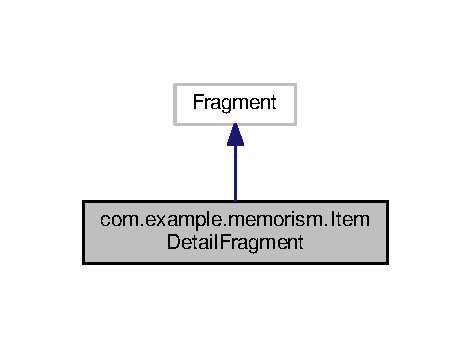
\includegraphics[width=226pt]{d1/db4/classcom_1_1example_1_1memorism_1_1_item_detail_fragment__inherit__graph}
\end{center}
\end{figure}


Collaboration diagram for com.\+example.\+memorism.\+Item\+Detail\+Fragment\+:
\nopagebreak
\begin{figure}[H]
\begin{center}
\leavevmode
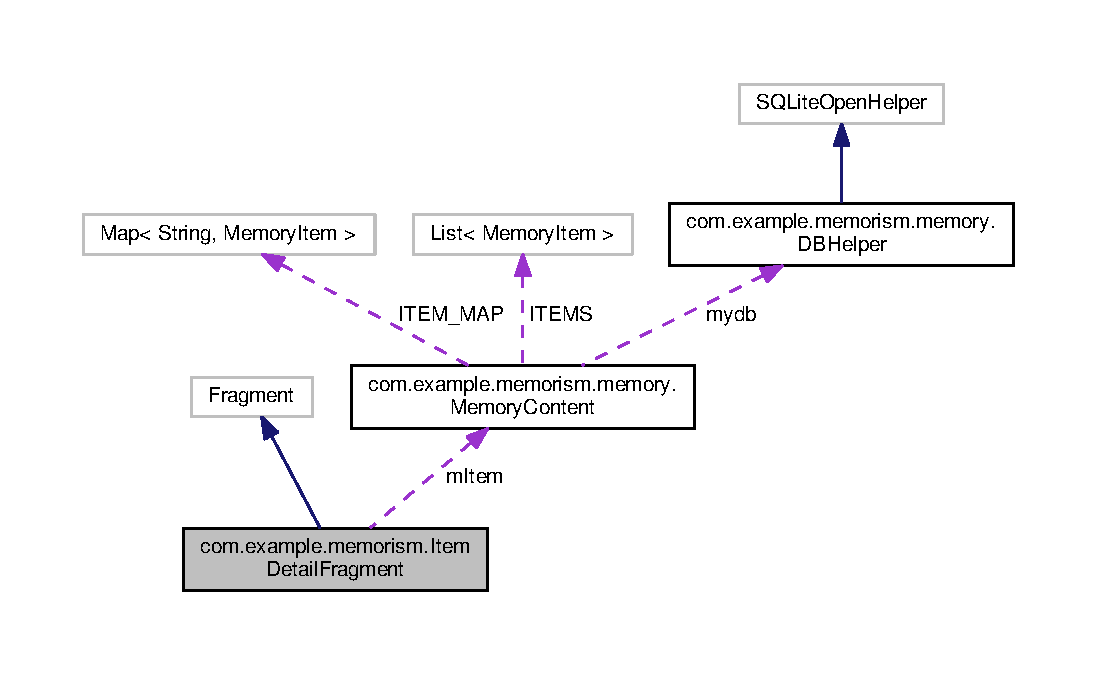
\includegraphics[width=350pt]{de/d74/classcom_1_1example_1_1memorism_1_1_item_detail_fragment__coll__graph}
\end{center}
\end{figure}
\subsection*{Public Member Functions}
\begin{DoxyCompactItemize}
\item 
\hyperlink{classcom_1_1example_1_1memorism_1_1_item_detail_fragment_abe2ebd5db13c9ea5fae5fc6aef4fd1f0}{Item\+Detail\+Fragment} ()
\item 
void \hyperlink{classcom_1_1example_1_1memorism_1_1_item_detail_fragment_ad7e424057935edb269914905533dc75b}{on\+Create} (Bundle saved\+Instance\+State)
\item 
View \hyperlink{classcom_1_1example_1_1memorism_1_1_item_detail_fragment_a7344c27a8c7f8fdafd6d91bb0a6d1b2b}{on\+Create\+View} (Layout\+Inflater inflater, View\+Group container, Bundle saved\+Instance\+State)
\end{DoxyCompactItemize}
\subsection*{Static Public Attributes}
\begin{DoxyCompactItemize}
\item 
static final String \hyperlink{classcom_1_1example_1_1memorism_1_1_item_detail_fragment_a580108a1952bf48a351a80530dd5223c}{A\+R\+G\+\_\+\+I\+T\+E\+M\+\_\+\+ID} = \char`\"{}item\+\_\+id\char`\"{}
\item 
static Memory\+Content.\+Memory\+Item \hyperlink{classcom_1_1example_1_1memorism_1_1_item_detail_fragment_ac763290f824e91141020dc2a61e424b4}{m\+Item}
\end{DoxyCompactItemize}


\subsection{Detailed Description}
A fragment representing a single Item detail screen. This fragment is either contained in a \hyperlink{classcom_1_1example_1_1memorism_1_1_item_list_activity}{Item\+List\+Activity} in two-\/pane mode (on tablets) or a \hyperlink{classcom_1_1example_1_1memorism_1_1_item_detail_activity}{Item\+Detail\+Activity} on handsets. 

Definition at line 20 of file Item\+Detail\+Fragment.\+java.



\subsection{Constructor \& Destructor Documentation}
\index{com\+::example\+::memorism\+::\+Item\+Detail\+Fragment@{com\+::example\+::memorism\+::\+Item\+Detail\+Fragment}!Item\+Detail\+Fragment@{Item\+Detail\+Fragment}}
\index{Item\+Detail\+Fragment@{Item\+Detail\+Fragment}!com\+::example\+::memorism\+::\+Item\+Detail\+Fragment@{com\+::example\+::memorism\+::\+Item\+Detail\+Fragment}}
\subsubsection[{\texorpdfstring{Item\+Detail\+Fragment()}{ItemDetailFragment()}}]{\setlength{\rightskip}{0pt plus 5cm}com.\+example.\+memorism.\+Item\+Detail\+Fragment.\+Item\+Detail\+Fragment (
\begin{DoxyParamCaption}
{}
\end{DoxyParamCaption}
)}\hypertarget{classcom_1_1example_1_1memorism_1_1_item_detail_fragment_abe2ebd5db13c9ea5fae5fc6aef4fd1f0}{}\label{classcom_1_1example_1_1memorism_1_1_item_detail_fragment_abe2ebd5db13c9ea5fae5fc6aef4fd1f0}
Mandatory empty constructor for the fragment manager to instantiate the fragment (e.\+g. upon screen orientation changes). 

Definition at line 36 of file Item\+Detail\+Fragment.\+java.



\subsection{Member Function Documentation}
\index{com\+::example\+::memorism\+::\+Item\+Detail\+Fragment@{com\+::example\+::memorism\+::\+Item\+Detail\+Fragment}!on\+Create@{on\+Create}}
\index{on\+Create@{on\+Create}!com\+::example\+::memorism\+::\+Item\+Detail\+Fragment@{com\+::example\+::memorism\+::\+Item\+Detail\+Fragment}}
\subsubsection[{\texorpdfstring{on\+Create(\+Bundle saved\+Instance\+State)}{onCreate(Bundle savedInstanceState)}}]{\setlength{\rightskip}{0pt plus 5cm}void com.\+example.\+memorism.\+Item\+Detail\+Fragment.\+on\+Create (
\begin{DoxyParamCaption}
\item[{Bundle}]{saved\+Instance\+State}
\end{DoxyParamCaption}
)}\hypertarget{classcom_1_1example_1_1memorism_1_1_item_detail_fragment_ad7e424057935edb269914905533dc75b}{}\label{classcom_1_1example_1_1memorism_1_1_item_detail_fragment_ad7e424057935edb269914905533dc75b}


Definition at line 40 of file Item\+Detail\+Fragment.\+java.

\index{com\+::example\+::memorism\+::\+Item\+Detail\+Fragment@{com\+::example\+::memorism\+::\+Item\+Detail\+Fragment}!on\+Create\+View@{on\+Create\+View}}
\index{on\+Create\+View@{on\+Create\+View}!com\+::example\+::memorism\+::\+Item\+Detail\+Fragment@{com\+::example\+::memorism\+::\+Item\+Detail\+Fragment}}
\subsubsection[{\texorpdfstring{on\+Create\+View(\+Layout\+Inflater inflater, View\+Group container, Bundle saved\+Instance\+State)}{onCreateView(LayoutInflater inflater, ViewGroup container, Bundle savedInstanceState)}}]{\setlength{\rightskip}{0pt plus 5cm}View com.\+example.\+memorism.\+Item\+Detail\+Fragment.\+on\+Create\+View (
\begin{DoxyParamCaption}
\item[{Layout\+Inflater}]{inflater, }
\item[{View\+Group}]{container, }
\item[{Bundle}]{saved\+Instance\+State}
\end{DoxyParamCaption}
)}\hypertarget{classcom_1_1example_1_1memorism_1_1_item_detail_fragment_a7344c27a8c7f8fdafd6d91bb0a6d1b2b}{}\label{classcom_1_1example_1_1memorism_1_1_item_detail_fragment_a7344c27a8c7f8fdafd6d91bb0a6d1b2b}


Definition at line 58 of file Item\+Detail\+Fragment.\+java.



\subsection{Member Data Documentation}
\index{com\+::example\+::memorism\+::\+Item\+Detail\+Fragment@{com\+::example\+::memorism\+::\+Item\+Detail\+Fragment}!A\+R\+G\+\_\+\+I\+T\+E\+M\+\_\+\+ID@{A\+R\+G\+\_\+\+I\+T\+E\+M\+\_\+\+ID}}
\index{A\+R\+G\+\_\+\+I\+T\+E\+M\+\_\+\+ID@{A\+R\+G\+\_\+\+I\+T\+E\+M\+\_\+\+ID}!com\+::example\+::memorism\+::\+Item\+Detail\+Fragment@{com\+::example\+::memorism\+::\+Item\+Detail\+Fragment}}
\subsubsection[{\texorpdfstring{A\+R\+G\+\_\+\+I\+T\+E\+M\+\_\+\+ID}{ARG_ITEM_ID}}]{\setlength{\rightskip}{0pt plus 5cm}final String com.\+example.\+memorism.\+Item\+Detail\+Fragment.\+A\+R\+G\+\_\+\+I\+T\+E\+M\+\_\+\+ID = \char`\"{}item\+\_\+id\char`\"{}\hspace{0.3cm}{\ttfamily [static]}}\hypertarget{classcom_1_1example_1_1memorism_1_1_item_detail_fragment_a580108a1952bf48a351a80530dd5223c}{}\label{classcom_1_1example_1_1memorism_1_1_item_detail_fragment_a580108a1952bf48a351a80530dd5223c}
The fragment argument representing the item ID that this fragment represents. 

Definition at line 25 of file Item\+Detail\+Fragment.\+java.

\index{com\+::example\+::memorism\+::\+Item\+Detail\+Fragment@{com\+::example\+::memorism\+::\+Item\+Detail\+Fragment}!m\+Item@{m\+Item}}
\index{m\+Item@{m\+Item}!com\+::example\+::memorism\+::\+Item\+Detail\+Fragment@{com\+::example\+::memorism\+::\+Item\+Detail\+Fragment}}
\subsubsection[{\texorpdfstring{m\+Item}{mItem}}]{\setlength{\rightskip}{0pt plus 5cm}Memory\+Content.\+Memory\+Item com.\+example.\+memorism.\+Item\+Detail\+Fragment.\+m\+Item\hspace{0.3cm}{\ttfamily [static]}}\hypertarget{classcom_1_1example_1_1memorism_1_1_item_detail_fragment_ac763290f824e91141020dc2a61e424b4}{}\label{classcom_1_1example_1_1memorism_1_1_item_detail_fragment_ac763290f824e91141020dc2a61e424b4}
The dummy title this fragment is presenting. 

Definition at line 30 of file Item\+Detail\+Fragment.\+java.



The documentation for this class was generated from the following file\+:\begin{DoxyCompactItemize}
\item 
/home/farid/\+Android\+Studio\+Projects/\+Memorism/app/src/main/java/com/example/memorism/\hyperlink{_item_detail_fragment_8java}{Item\+Detail\+Fragment.\+java}\end{DoxyCompactItemize}

\hypertarget{classcom_1_1example_1_1memorism_1_1_item_list_activity}{}\section{com.\+example.\+memorism.\+Item\+List\+Activity Class Reference}
\label{classcom_1_1example_1_1memorism_1_1_item_list_activity}\index{com.\+example.\+memorism.\+Item\+List\+Activity@{com.\+example.\+memorism.\+Item\+List\+Activity}}


Inheritance diagram for com.\+example.\+memorism.\+Item\+List\+Activity\+:\nopagebreak
\begin{figure}[H]
\begin{center}
\leavevmode
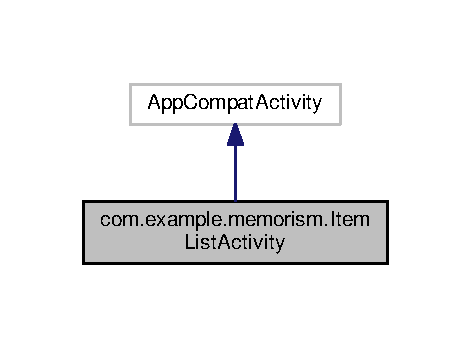
\includegraphics[width=226pt]{d8/d6d/classcom_1_1example_1_1memorism_1_1_item_list_activity__inherit__graph}
\end{center}
\end{figure}


Collaboration diagram for com.\+example.\+memorism.\+Item\+List\+Activity\+:\nopagebreak
\begin{figure}[H]
\begin{center}
\leavevmode
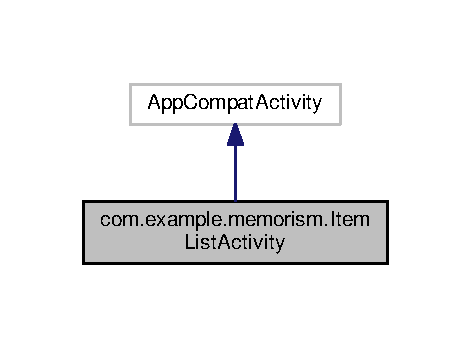
\includegraphics[width=226pt]{d2/d58/classcom_1_1example_1_1memorism_1_1_item_list_activity__coll__graph}
\end{center}
\end{figure}
\subsection*{Classes}
\begin{DoxyCompactItemize}
\item 
class {\bfseries Simple\+Item\+Recycler\+View\+Adapter}
\end{DoxyCompactItemize}
\subsection*{Protected Member Functions}
\begin{DoxyCompactItemize}
\item 
void \hyperlink{classcom_1_1example_1_1memorism_1_1_item_list_activity_a77070a24ee8e96e2283a9383b352ed6f}{on\+Create} (Bundle saved\+Instance\+State)
\end{DoxyCompactItemize}


\subsection{Detailed Description}
An activity representing a list of Items. This activity has different presentations for handset and tablet-\/size devices. On handsets, the activity presents a list of items, which when touched, lead to a \hyperlink{classcom_1_1example_1_1memorism_1_1_item_detail_activity}{Item\+Detail\+Activity} representing item details. On tablets, the activity presents the list of items and item details side-\/by-\/side using two vertical panes. 

Definition at line 30 of file Item\+List\+Activity.\+java.



\subsection{Member Function Documentation}
\index{com\+::example\+::memorism\+::\+Item\+List\+Activity@{com\+::example\+::memorism\+::\+Item\+List\+Activity}!on\+Create@{on\+Create}}
\index{on\+Create@{on\+Create}!com\+::example\+::memorism\+::\+Item\+List\+Activity@{com\+::example\+::memorism\+::\+Item\+List\+Activity}}
\subsubsection[{\texorpdfstring{on\+Create(\+Bundle saved\+Instance\+State)}{onCreate(Bundle savedInstanceState)}}]{\setlength{\rightskip}{0pt plus 5cm}void com.\+example.\+memorism.\+Item\+List\+Activity.\+on\+Create (
\begin{DoxyParamCaption}
\item[{Bundle}]{saved\+Instance\+State}
\end{DoxyParamCaption}
)\hspace{0.3cm}{\ttfamily [protected]}}\hypertarget{classcom_1_1example_1_1memorism_1_1_item_list_activity_a77070a24ee8e96e2283a9383b352ed6f}{}\label{classcom_1_1example_1_1memorism_1_1_item_list_activity_a77070a24ee8e96e2283a9383b352ed6f}


Definition at line 39 of file Item\+List\+Activity.\+java.



The documentation for this class was generated from the following file\+:\begin{DoxyCompactItemize}
\item 
/home/farid/\+Android\+Studio\+Projects/\+Memorism/app/src/main/java/com/example/memorism/\hyperlink{_item_list_activity_8java}{Item\+List\+Activity.\+java}\end{DoxyCompactItemize}

\hypertarget{classcom_1_1example_1_1memorism_1_1_main_menu}{}\section{com.\+example.\+memorism.\+Main\+Menu Class Reference}
\label{classcom_1_1example_1_1memorism_1_1_main_menu}\index{com.\+example.\+memorism.\+Main\+Menu@{com.\+example.\+memorism.\+Main\+Menu}}


Inheritance diagram for com.\+example.\+memorism.\+Main\+Menu\+:\nopagebreak
\begin{figure}[H]
\begin{center}
\leavevmode
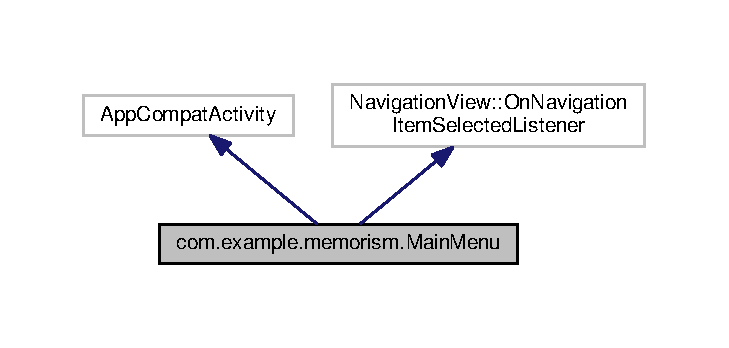
\includegraphics[width=350pt]{de/ddb/classcom_1_1example_1_1memorism_1_1_main_menu__inherit__graph}
\end{center}
\end{figure}


Collaboration diagram for com.\+example.\+memorism.\+Main\+Menu\+:\nopagebreak
\begin{figure}[H]
\begin{center}
\leavevmode
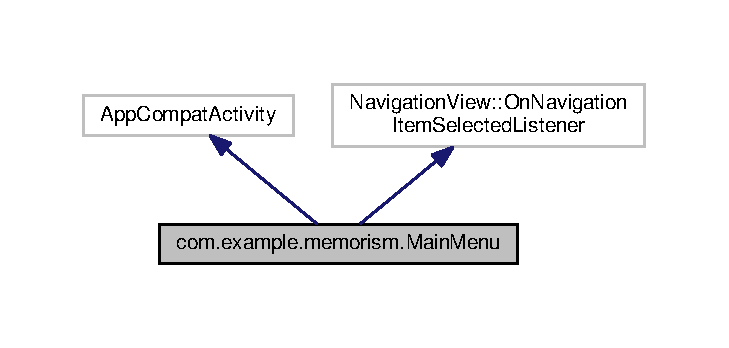
\includegraphics[width=350pt]{d0/d04/classcom_1_1example_1_1memorism_1_1_main_menu__coll__graph}
\end{center}
\end{figure}
\subsection*{Public Member Functions}
\begin{DoxyCompactItemize}
\item 
void \hyperlink{classcom_1_1example_1_1memorism_1_1_main_menu_a95779c69310377bd8a179729860b8378}{on\+Back\+Pressed} ()
\item 
boolean \hyperlink{classcom_1_1example_1_1memorism_1_1_main_menu_acb3ffdf12dfd08e510ce6aa55c65b52c}{on\+Create\+Options\+Menu} (Menu menu)
\item 
boolean \hyperlink{classcom_1_1example_1_1memorism_1_1_main_menu_a6af03ac2a8ca72dc6b763caab4707bad}{on\+Options\+Item\+Selected} (Menu\+Item item)
\item 
boolean \hyperlink{classcom_1_1example_1_1memorism_1_1_main_menu_a49832e3cb7178b6f317a38cd88f05bf2}{on\+Navigation\+Item\+Selected} (Menu\+Item item)
\end{DoxyCompactItemize}
\subsection*{Protected Member Functions}
\begin{DoxyCompactItemize}
\item 
void \hyperlink{classcom_1_1example_1_1memorism_1_1_main_menu_ab8ad80a15fae9ec3ade6b9ce0a108435}{on\+Start} ()
\item 
void \hyperlink{classcom_1_1example_1_1memorism_1_1_main_menu_a1739715a74237054762ff983fadeed4d}{on\+Create} (Bundle saved\+Instance\+State)
\end{DoxyCompactItemize}


\subsection{Detailed Description}


Definition at line 25 of file Main\+Menu.\+java.



\subsection{Member Function Documentation}
\index{com\+::example\+::memorism\+::\+Main\+Menu@{com\+::example\+::memorism\+::\+Main\+Menu}!on\+Back\+Pressed@{on\+Back\+Pressed}}
\index{on\+Back\+Pressed@{on\+Back\+Pressed}!com\+::example\+::memorism\+::\+Main\+Menu@{com\+::example\+::memorism\+::\+Main\+Menu}}
\subsubsection[{\texorpdfstring{on\+Back\+Pressed()}{onBackPressed()}}]{\setlength{\rightskip}{0pt plus 5cm}void com.\+example.\+memorism.\+Main\+Menu.\+on\+Back\+Pressed (
\begin{DoxyParamCaption}
{}
\end{DoxyParamCaption}
)}\hypertarget{classcom_1_1example_1_1memorism_1_1_main_menu_a95779c69310377bd8a179729860b8378}{}\label{classcom_1_1example_1_1memorism_1_1_main_menu_a95779c69310377bd8a179729860b8378}


Definition at line 75 of file Main\+Menu.\+java.

\index{com\+::example\+::memorism\+::\+Main\+Menu@{com\+::example\+::memorism\+::\+Main\+Menu}!on\+Create@{on\+Create}}
\index{on\+Create@{on\+Create}!com\+::example\+::memorism\+::\+Main\+Menu@{com\+::example\+::memorism\+::\+Main\+Menu}}
\subsubsection[{\texorpdfstring{on\+Create(\+Bundle saved\+Instance\+State)}{onCreate(Bundle savedInstanceState)}}]{\setlength{\rightskip}{0pt plus 5cm}void com.\+example.\+memorism.\+Main\+Menu.\+on\+Create (
\begin{DoxyParamCaption}
\item[{Bundle}]{saved\+Instance\+State}
\end{DoxyParamCaption}
)\hspace{0.3cm}{\ttfamily [protected]}}\hypertarget{classcom_1_1example_1_1memorism_1_1_main_menu_a1739715a74237054762ff983fadeed4d}{}\label{classcom_1_1example_1_1memorism_1_1_main_menu_a1739715a74237054762ff983fadeed4d}


Definition at line 37 of file Main\+Menu.\+java.

\index{com\+::example\+::memorism\+::\+Main\+Menu@{com\+::example\+::memorism\+::\+Main\+Menu}!on\+Create\+Options\+Menu@{on\+Create\+Options\+Menu}}
\index{on\+Create\+Options\+Menu@{on\+Create\+Options\+Menu}!com\+::example\+::memorism\+::\+Main\+Menu@{com\+::example\+::memorism\+::\+Main\+Menu}}
\subsubsection[{\texorpdfstring{on\+Create\+Options\+Menu(\+Menu menu)}{onCreateOptionsMenu(Menu menu)}}]{\setlength{\rightskip}{0pt plus 5cm}boolean com.\+example.\+memorism.\+Main\+Menu.\+on\+Create\+Options\+Menu (
\begin{DoxyParamCaption}
\item[{Menu}]{menu}
\end{DoxyParamCaption}
)}\hypertarget{classcom_1_1example_1_1memorism_1_1_main_menu_acb3ffdf12dfd08e510ce6aa55c65b52c}{}\label{classcom_1_1example_1_1memorism_1_1_main_menu_acb3ffdf12dfd08e510ce6aa55c65b52c}


Definition at line 85 of file Main\+Menu.\+java.

\index{com\+::example\+::memorism\+::\+Main\+Menu@{com\+::example\+::memorism\+::\+Main\+Menu}!on\+Navigation\+Item\+Selected@{on\+Navigation\+Item\+Selected}}
\index{on\+Navigation\+Item\+Selected@{on\+Navigation\+Item\+Selected}!com\+::example\+::memorism\+::\+Main\+Menu@{com\+::example\+::memorism\+::\+Main\+Menu}}
\subsubsection[{\texorpdfstring{on\+Navigation\+Item\+Selected(\+Menu\+Item item)}{onNavigationItemSelected(MenuItem item)}}]{\setlength{\rightskip}{0pt plus 5cm}boolean com.\+example.\+memorism.\+Main\+Menu.\+on\+Navigation\+Item\+Selected (
\begin{DoxyParamCaption}
\item[{Menu\+Item}]{item}
\end{DoxyParamCaption}
)}\hypertarget{classcom_1_1example_1_1memorism_1_1_main_menu_a49832e3cb7178b6f317a38cd88f05bf2}{}\label{classcom_1_1example_1_1memorism_1_1_main_menu_a49832e3cb7178b6f317a38cd88f05bf2}


Definition at line 108 of file Main\+Menu.\+java.

\index{com\+::example\+::memorism\+::\+Main\+Menu@{com\+::example\+::memorism\+::\+Main\+Menu}!on\+Options\+Item\+Selected@{on\+Options\+Item\+Selected}}
\index{on\+Options\+Item\+Selected@{on\+Options\+Item\+Selected}!com\+::example\+::memorism\+::\+Main\+Menu@{com\+::example\+::memorism\+::\+Main\+Menu}}
\subsubsection[{\texorpdfstring{on\+Options\+Item\+Selected(\+Menu\+Item item)}{onOptionsItemSelected(MenuItem item)}}]{\setlength{\rightskip}{0pt plus 5cm}boolean com.\+example.\+memorism.\+Main\+Menu.\+on\+Options\+Item\+Selected (
\begin{DoxyParamCaption}
\item[{Menu\+Item}]{item}
\end{DoxyParamCaption}
)}\hypertarget{classcom_1_1example_1_1memorism_1_1_main_menu_a6af03ac2a8ca72dc6b763caab4707bad}{}\label{classcom_1_1example_1_1memorism_1_1_main_menu_a6af03ac2a8ca72dc6b763caab4707bad}


Definition at line 92 of file Main\+Menu.\+java.

\index{com\+::example\+::memorism\+::\+Main\+Menu@{com\+::example\+::memorism\+::\+Main\+Menu}!on\+Start@{on\+Start}}
\index{on\+Start@{on\+Start}!com\+::example\+::memorism\+::\+Main\+Menu@{com\+::example\+::memorism\+::\+Main\+Menu}}
\subsubsection[{\texorpdfstring{on\+Start()}{onStart()}}]{\setlength{\rightskip}{0pt plus 5cm}void com.\+example.\+memorism.\+Main\+Menu.\+on\+Start (
\begin{DoxyParamCaption}
{}
\end{DoxyParamCaption}
)\hspace{0.3cm}{\ttfamily [protected]}}\hypertarget{classcom_1_1example_1_1memorism_1_1_main_menu_ab8ad80a15fae9ec3ade6b9ce0a108435}{}\label{classcom_1_1example_1_1memorism_1_1_main_menu_ab8ad80a15fae9ec3ade6b9ce0a108435}


Definition at line 31 of file Main\+Menu.\+java.



The documentation for this class was generated from the following file\+:\begin{DoxyCompactItemize}
\item 
/home/farid/\+Android\+Studio\+Projects/\+Memorism/app/src/main/java/com/example/memorism/\hyperlink{_main_menu_8java}{Main\+Menu.\+java}\end{DoxyCompactItemize}

\hypertarget{classcom_1_1example_1_1memorism_1_1memory_1_1_memory_content}{}\section{com.\+example.\+memorism.\+memory.\+Memory\+Content Class Reference}
\label{classcom_1_1example_1_1memorism_1_1memory_1_1_memory_content}\index{com.\+example.\+memorism.\+memory.\+Memory\+Content@{com.\+example.\+memorism.\+memory.\+Memory\+Content}}


Collaboration diagram for com.\+example.\+memorism.\+memory.\+Memory\+Content\+:
% FIG 0
\subsection*{Classes}
\begin{DoxyCompactItemize}
\item 
class {\bfseries Memory\+Item}
\end{DoxyCompactItemize}
\subsection*{Static Public Member Functions}
\begin{DoxyCompactItemize}
\item 
static List$<$ String $>$ \hyperlink{classcom_1_1example_1_1memorism_1_1memory_1_1_memory_content_abee14d3117afebf9c4dbbe4e42a67681}{get\+All\+Trip\+Name} ()
\item 
static List$<$ Memory\+Item $>$ \hyperlink{classcom_1_1example_1_1memorism_1_1memory_1_1_memory_content_a344d7fd205ff5645a7b0e37d71006ef0}{get\+Item\+Trip} (String name)
\item 
static void \hyperlink{classcom_1_1example_1_1memorism_1_1memory_1_1_memory_content_aa4de84ed8cc74b2a05eee78be9006beb}{add\+Item} (Memory\+Item item)
\item 
static void \hyperlink{classcom_1_1example_1_1memorism_1_1memory_1_1_memory_content_a830cbb9924e5992dccb310b7d3ef484d}{add\+Item} (String trip\+\_\+name, String date, String title, String details, double positionX, double positionY)
\item 
static void \hyperlink{classcom_1_1example_1_1memorism_1_1memory_1_1_memory_content_a0712c96d927ddb6c68202f9ea24bea5c}{remove\+Item} (Memory\+Item item)
\item 
static void \hyperlink{classcom_1_1example_1_1memorism_1_1memory_1_1_memory_content_a4641b5327eb70f1d7754d77aa71bfe0b}{remove\+Trip} (String name)
\item 
static String \hyperlink{classcom_1_1example_1_1memorism_1_1memory_1_1_memory_content_a4e7cf028fd6d81395968bc10f42a7643}{make\+Details} (Memory\+Item item)
\end{DoxyCompactItemize}
\subsection*{Static Public Attributes}
\begin{DoxyCompactItemize}
\item 
static final List$<$ Memory\+Item $>$ \hyperlink{classcom_1_1example_1_1memorism_1_1memory_1_1_memory_content_a1bcc45e0adac63b034f3459da2efcf56}{I\+T\+E\+MS} = new Array\+List$<$Memory\+Item$>$()
\item 
static \hyperlink{classcom_1_1example_1_1memorism_1_1memory_1_1_d_b_helper}{D\+B\+Helper} \hyperlink{classcom_1_1example_1_1memorism_1_1memory_1_1_memory_content_ae0b89ca96c4bb6c8544e45feebdee2df}{mydb}
\item 
static final Map$<$ String, Memory\+Item $>$ \hyperlink{classcom_1_1example_1_1memorism_1_1memory_1_1_memory_content_a0699740b06818cb8000d1e01c1531a00}{I\+T\+E\+M\+\_\+\+M\+AP} = new Hash\+Map$<$String, Memory\+Item$>$()
\item 
static String \hyperlink{classcom_1_1example_1_1memorism_1_1memory_1_1_memory_content_aaa05c280eab2d10c9902b19a03825952}{trip\+\_\+name\+\_\+prompted} = \char`\"{}\char`\"{}
\end{DoxyCompactItemize}


\subsection{Detailed Description}
Helper class for providing sample title for user interfaces created by Android template wizards. 

T\+O\+DO\+: Replace all uses of this class before publishing your app. 

Definition at line 21 of file Memory\+Content.\+java.



\subsection{Member Function Documentation}
\index{com\+::example\+::memorism\+::memory\+::\+Memory\+Content@{com\+::example\+::memorism\+::memory\+::\+Memory\+Content}!add\+Item@{add\+Item}}
\index{add\+Item@{add\+Item}!com\+::example\+::memorism\+::memory\+::\+Memory\+Content@{com\+::example\+::memorism\+::memory\+::\+Memory\+Content}}
\subsubsection[{\texorpdfstring{add\+Item(\+Memory\+Item item)}{addItem(MemoryItem item)}}]{\setlength{\rightskip}{0pt plus 5cm}static void com.\+example.\+memorism.\+memory.\+Memory\+Content.\+add\+Item (
\begin{DoxyParamCaption}
\item[{Memory\+Item}]{item}
\end{DoxyParamCaption}
)\hspace{0.3cm}{\ttfamily [static]}}\hypertarget{classcom_1_1example_1_1memorism_1_1memory_1_1_memory_content_aa4de84ed8cc74b2a05eee78be9006beb}{}\label{classcom_1_1example_1_1memorism_1_1memory_1_1_memory_content_aa4de84ed8cc74b2a05eee78be9006beb}


Definition at line 61 of file Memory\+Content.\+java.

\index{com\+::example\+::memorism\+::memory\+::\+Memory\+Content@{com\+::example\+::memorism\+::memory\+::\+Memory\+Content}!add\+Item@{add\+Item}}
\index{add\+Item@{add\+Item}!com\+::example\+::memorism\+::memory\+::\+Memory\+Content@{com\+::example\+::memorism\+::memory\+::\+Memory\+Content}}
\subsubsection[{\texorpdfstring{add\+Item(\+String trip\+\_\+name, String date, String title, String details, double position\+X, double position\+Y)}{addItem(String trip_name, String date, String title, String details, double positionX, double positionY)}}]{\setlength{\rightskip}{0pt plus 5cm}static void com.\+example.\+memorism.\+memory.\+Memory\+Content.\+add\+Item (
\begin{DoxyParamCaption}
\item[{String}]{trip\+\_\+name, }
\item[{String}]{date, }
\item[{String}]{title, }
\item[{String}]{details, }
\item[{double}]{positionX, }
\item[{double}]{positionY}
\end{DoxyParamCaption}
)\hspace{0.3cm}{\ttfamily [static]}}\hypertarget{classcom_1_1example_1_1memorism_1_1memory_1_1_memory_content_a830cbb9924e5992dccb310b7d3ef484d}{}\label{classcom_1_1example_1_1memorism_1_1memory_1_1_memory_content_a830cbb9924e5992dccb310b7d3ef484d}


Definition at line 67 of file Memory\+Content.\+java.

\index{com\+::example\+::memorism\+::memory\+::\+Memory\+Content@{com\+::example\+::memorism\+::memory\+::\+Memory\+Content}!get\+All\+Trip\+Name@{get\+All\+Trip\+Name}}
\index{get\+All\+Trip\+Name@{get\+All\+Trip\+Name}!com\+::example\+::memorism\+::memory\+::\+Memory\+Content@{com\+::example\+::memorism\+::memory\+::\+Memory\+Content}}
\subsubsection[{\texorpdfstring{get\+All\+Trip\+Name()}{getAllTripName()}}]{\setlength{\rightskip}{0pt plus 5cm}static List$<$String$>$ com.\+example.\+memorism.\+memory.\+Memory\+Content.\+get\+All\+Trip\+Name (
\begin{DoxyParamCaption}
{}
\end{DoxyParamCaption}
)\hspace{0.3cm}{\ttfamily [static]}}\hypertarget{classcom_1_1example_1_1memorism_1_1memory_1_1_memory_content_abee14d3117afebf9c4dbbe4e42a67681}{}\label{classcom_1_1example_1_1memorism_1_1memory_1_1_memory_content_abee14d3117afebf9c4dbbe4e42a67681}


Definition at line 35 of file Memory\+Content.\+java.

\index{com\+::example\+::memorism\+::memory\+::\+Memory\+Content@{com\+::example\+::memorism\+::memory\+::\+Memory\+Content}!get\+Item\+Trip@{get\+Item\+Trip}}
\index{get\+Item\+Trip@{get\+Item\+Trip}!com\+::example\+::memorism\+::memory\+::\+Memory\+Content@{com\+::example\+::memorism\+::memory\+::\+Memory\+Content}}
\subsubsection[{\texorpdfstring{get\+Item\+Trip(\+String name)}{getItemTrip(String name)}}]{\setlength{\rightskip}{0pt plus 5cm}static List$<$Memory\+Item$>$ com.\+example.\+memorism.\+memory.\+Memory\+Content.\+get\+Item\+Trip (
\begin{DoxyParamCaption}
\item[{String}]{name}
\end{DoxyParamCaption}
)\hspace{0.3cm}{\ttfamily [static]}}\hypertarget{classcom_1_1example_1_1memorism_1_1memory_1_1_memory_content_a344d7fd205ff5645a7b0e37d71006ef0}{}\label{classcom_1_1example_1_1memorism_1_1memory_1_1_memory_content_a344d7fd205ff5645a7b0e37d71006ef0}


Definition at line 49 of file Memory\+Content.\+java.

\index{com\+::example\+::memorism\+::memory\+::\+Memory\+Content@{com\+::example\+::memorism\+::memory\+::\+Memory\+Content}!make\+Details@{make\+Details}}
\index{make\+Details@{make\+Details}!com\+::example\+::memorism\+::memory\+::\+Memory\+Content@{com\+::example\+::memorism\+::memory\+::\+Memory\+Content}}
\subsubsection[{\texorpdfstring{make\+Details(\+Memory\+Item item)}{makeDetails(MemoryItem item)}}]{\setlength{\rightskip}{0pt plus 5cm}static String com.\+example.\+memorism.\+memory.\+Memory\+Content.\+make\+Details (
\begin{DoxyParamCaption}
\item[{Memory\+Item}]{item}
\end{DoxyParamCaption}
)\hspace{0.3cm}{\ttfamily [static]}}\hypertarget{classcom_1_1example_1_1memorism_1_1memory_1_1_memory_content_a4e7cf028fd6d81395968bc10f42a7643}{}\label{classcom_1_1example_1_1memorism_1_1memory_1_1_memory_content_a4e7cf028fd6d81395968bc10f42a7643}


Definition at line 91 of file Memory\+Content.\+java.

\index{com\+::example\+::memorism\+::memory\+::\+Memory\+Content@{com\+::example\+::memorism\+::memory\+::\+Memory\+Content}!remove\+Item@{remove\+Item}}
\index{remove\+Item@{remove\+Item}!com\+::example\+::memorism\+::memory\+::\+Memory\+Content@{com\+::example\+::memorism\+::memory\+::\+Memory\+Content}}
\subsubsection[{\texorpdfstring{remove\+Item(\+Memory\+Item item)}{removeItem(MemoryItem item)}}]{\setlength{\rightskip}{0pt plus 5cm}static void com.\+example.\+memorism.\+memory.\+Memory\+Content.\+remove\+Item (
\begin{DoxyParamCaption}
\item[{Memory\+Item}]{item}
\end{DoxyParamCaption}
)\hspace{0.3cm}{\ttfamily [static]}}\hypertarget{classcom_1_1example_1_1memorism_1_1memory_1_1_memory_content_a0712c96d927ddb6c68202f9ea24bea5c}{}\label{classcom_1_1example_1_1memorism_1_1memory_1_1_memory_content_a0712c96d927ddb6c68202f9ea24bea5c}


Definition at line 76 of file Memory\+Content.\+java.

\index{com\+::example\+::memorism\+::memory\+::\+Memory\+Content@{com\+::example\+::memorism\+::memory\+::\+Memory\+Content}!remove\+Trip@{remove\+Trip}}
\index{remove\+Trip@{remove\+Trip}!com\+::example\+::memorism\+::memory\+::\+Memory\+Content@{com\+::example\+::memorism\+::memory\+::\+Memory\+Content}}
\subsubsection[{\texorpdfstring{remove\+Trip(\+String name)}{removeTrip(String name)}}]{\setlength{\rightskip}{0pt plus 5cm}static void com.\+example.\+memorism.\+memory.\+Memory\+Content.\+remove\+Trip (
\begin{DoxyParamCaption}
\item[{String}]{name}
\end{DoxyParamCaption}
)\hspace{0.3cm}{\ttfamily [static]}}\hypertarget{classcom_1_1example_1_1memorism_1_1memory_1_1_memory_content_a4641b5327eb70f1d7754d77aa71bfe0b}{}\label{classcom_1_1example_1_1memorism_1_1memory_1_1_memory_content_a4641b5327eb70f1d7754d77aa71bfe0b}


Definition at line 82 of file Memory\+Content.\+java.



\subsection{Member Data Documentation}
\index{com\+::example\+::memorism\+::memory\+::\+Memory\+Content@{com\+::example\+::memorism\+::memory\+::\+Memory\+Content}!I\+T\+E\+M\+\_\+\+M\+AP@{I\+T\+E\+M\+\_\+\+M\+AP}}
\index{I\+T\+E\+M\+\_\+\+M\+AP@{I\+T\+E\+M\+\_\+\+M\+AP}!com\+::example\+::memorism\+::memory\+::\+Memory\+Content@{com\+::example\+::memorism\+::memory\+::\+Memory\+Content}}
\subsubsection[{\texorpdfstring{I\+T\+E\+M\+\_\+\+M\+AP}{ITEM_MAP}}]{\setlength{\rightskip}{0pt plus 5cm}final Map$<$String, Memory\+Item$>$ com.\+example.\+memorism.\+memory.\+Memory\+Content.\+I\+T\+E\+M\+\_\+\+M\+AP = new Hash\+Map$<$String, Memory\+Item$>$()\hspace{0.3cm}{\ttfamily [static]}}\hypertarget{classcom_1_1example_1_1memorism_1_1memory_1_1_memory_content_a0699740b06818cb8000d1e01c1531a00}{}\label{classcom_1_1example_1_1memorism_1_1memory_1_1_memory_content_a0699740b06818cb8000d1e01c1531a00}
A map of sample (dummy) items, by ID. 

Definition at line 31 of file Memory\+Content.\+java.

\index{com\+::example\+::memorism\+::memory\+::\+Memory\+Content@{com\+::example\+::memorism\+::memory\+::\+Memory\+Content}!I\+T\+E\+MS@{I\+T\+E\+MS}}
\index{I\+T\+E\+MS@{I\+T\+E\+MS}!com\+::example\+::memorism\+::memory\+::\+Memory\+Content@{com\+::example\+::memorism\+::memory\+::\+Memory\+Content}}
\subsubsection[{\texorpdfstring{I\+T\+E\+MS}{ITEMS}}]{\setlength{\rightskip}{0pt plus 5cm}final List$<$Memory\+Item$>$ com.\+example.\+memorism.\+memory.\+Memory\+Content.\+I\+T\+E\+MS = new Array\+List$<$Memory\+Item$>$()\hspace{0.3cm}{\ttfamily [static]}}\hypertarget{classcom_1_1example_1_1memorism_1_1memory_1_1_memory_content_a1bcc45e0adac63b034f3459da2efcf56}{}\label{classcom_1_1example_1_1memorism_1_1memory_1_1_memory_content_a1bcc45e0adac63b034f3459da2efcf56}
An array of sample (dummy) items. 

Definition at line 26 of file Memory\+Content.\+java.

\index{com\+::example\+::memorism\+::memory\+::\+Memory\+Content@{com\+::example\+::memorism\+::memory\+::\+Memory\+Content}!mydb@{mydb}}
\index{mydb@{mydb}!com\+::example\+::memorism\+::memory\+::\+Memory\+Content@{com\+::example\+::memorism\+::memory\+::\+Memory\+Content}}
\subsubsection[{\texorpdfstring{mydb}{mydb}}]{\setlength{\rightskip}{0pt plus 5cm}{\bf D\+B\+Helper} com.\+example.\+memorism.\+memory.\+Memory\+Content.\+mydb\hspace{0.3cm}{\ttfamily [static]}}\hypertarget{classcom_1_1example_1_1memorism_1_1memory_1_1_memory_content_ae0b89ca96c4bb6c8544e45feebdee2df}{}\label{classcom_1_1example_1_1memorism_1_1memory_1_1_memory_content_ae0b89ca96c4bb6c8544e45feebdee2df}


Definition at line 27 of file Memory\+Content.\+java.

\index{com\+::example\+::memorism\+::memory\+::\+Memory\+Content@{com\+::example\+::memorism\+::memory\+::\+Memory\+Content}!trip\+\_\+name\+\_\+prompted@{trip\+\_\+name\+\_\+prompted}}
\index{trip\+\_\+name\+\_\+prompted@{trip\+\_\+name\+\_\+prompted}!com\+::example\+::memorism\+::memory\+::\+Memory\+Content@{com\+::example\+::memorism\+::memory\+::\+Memory\+Content}}
\subsubsection[{\texorpdfstring{trip\+\_\+name\+\_\+prompted}{trip_name_prompted}}]{\setlength{\rightskip}{0pt plus 5cm}String com.\+example.\+memorism.\+memory.\+Memory\+Content.\+trip\+\_\+name\+\_\+prompted = \char`\"{}\char`\"{}\hspace{0.3cm}{\ttfamily [static]}}\hypertarget{classcom_1_1example_1_1memorism_1_1memory_1_1_memory_content_aaa05c280eab2d10c9902b19a03825952}{}\label{classcom_1_1example_1_1memorism_1_1memory_1_1_memory_content_aaa05c280eab2d10c9902b19a03825952}


Definition at line 33 of file Memory\+Content.\+java.



The documentation for this class was generated from the following file\+:\begin{DoxyCompactItemize}
\item 
/home/farid/\+Android\+Studio\+Projects/\+Memorism/app/src/main/java/com/example/memorism/memory/\hyperlink{_memory_content_8java}{Memory\+Content.\+java}\end{DoxyCompactItemize}

\hypertarget{classcom_1_1example_1_1memorism_1_1misc__funct}{}\section{com.\+example.\+memorism.\+misc\+\_\+funct Class Reference}
\label{classcom_1_1example_1_1memorism_1_1misc__funct}\index{com.\+example.\+memorism.\+misc\+\_\+funct@{com.\+example.\+memorism.\+misc\+\_\+funct}}
\subsection*{Static Public Member Functions}
\begin{DoxyCompactItemize}
\item 
static double \hyperlink{classcom_1_1example_1_1memorism_1_1misc__funct_a4ecdbe29cdf38a7e8b2552e68a3c27fb}{random\+Numberpos\+XY} (int min, int max)
\end{DoxyCompactItemize}


\subsection{Detailed Description}
Created by farid on 26/12/17. 

Definition at line 14 of file misc\+\_\+funct.\+java.



\subsection{Member Function Documentation}
\index{com\+::example\+::memorism\+::misc\+\_\+funct@{com\+::example\+::memorism\+::misc\+\_\+funct}!random\+Numberpos\+XY@{random\+Numberpos\+XY}}
\index{random\+Numberpos\+XY@{random\+Numberpos\+XY}!com\+::example\+::memorism\+::misc\+\_\+funct@{com\+::example\+::memorism\+::misc\+\_\+funct}}
\subsubsection[{\texorpdfstring{random\+Numberpos\+X\+Y(int min, int max)}{randomNumberposXY(int min, int max)}}]{\setlength{\rightskip}{0pt plus 5cm}static double com.\+example.\+memorism.\+misc\+\_\+funct.\+random\+Numberpos\+XY (
\begin{DoxyParamCaption}
\item[{int}]{min, }
\item[{int}]{max}
\end{DoxyParamCaption}
)\hspace{0.3cm}{\ttfamily [static]}}\hypertarget{classcom_1_1example_1_1memorism_1_1misc__funct_a4ecdbe29cdf38a7e8b2552e68a3c27fb}{}\label{classcom_1_1example_1_1memorism_1_1misc__funct_a4ecdbe29cdf38a7e8b2552e68a3c27fb}


Definition at line 16 of file misc\+\_\+funct.\+java.



The documentation for this class was generated from the following file\+:\begin{DoxyCompactItemize}
\item 
/home/farid/\+Android\+Studio\+Projects/\+Memorism/app/src/main/java/com/example/memorism/\hyperlink{misc__funct_8java}{misc\+\_\+funct.\+java}\end{DoxyCompactItemize}

\hypertarget{classcom_1_1example_1_1memorism_1_1_show___map}{}\section{com.\+example.\+memorism.\+Show\+\_\+\+Map Class Reference}
\label{classcom_1_1example_1_1memorism_1_1_show___map}\index{com.\+example.\+memorism.\+Show\+\_\+\+Map@{com.\+example.\+memorism.\+Show\+\_\+\+Map}}


Inheritance diagram for com.\+example.\+memorism.\+Show\+\_\+\+Map\+:
\nopagebreak
\begin{figure}[H]
\begin{center}
\leavevmode
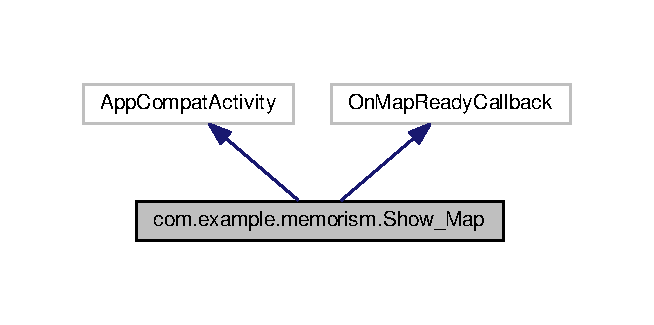
\includegraphics[width=314pt]{d5/dec/classcom_1_1example_1_1memorism_1_1_show___map__inherit__graph}
\end{center}
\end{figure}


Collaboration diagram for com.\+example.\+memorism.\+Show\+\_\+\+Map\+:
\nopagebreak
\begin{figure}[H]
\begin{center}
\leavevmode
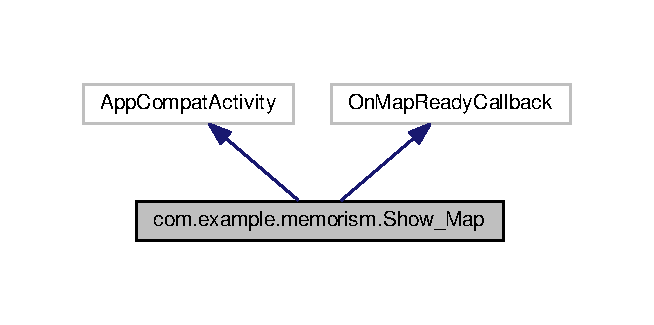
\includegraphics[width=314pt]{d3/ddc/classcom_1_1example_1_1memorism_1_1_show___map__coll__graph}
\end{center}
\end{figure}
\subsection*{Public Member Functions}
\begin{DoxyCompactItemize}
\item 
void \hyperlink{classcom_1_1example_1_1memorism_1_1_show___map_a1db450c9105bdeeb9cb57a6253d0cbc4}{on\+Map\+Ready} (Google\+Map google\+Map)
\end{DoxyCompactItemize}
\subsection*{Protected Member Functions}
\begin{DoxyCompactItemize}
\item 
void \hyperlink{classcom_1_1example_1_1memorism_1_1_show___map_a1f01cea0c30154354da65bef34090960}{on\+Create} (Bundle saved\+Instance\+State)
\end{DoxyCompactItemize}


\subsection{Detailed Description}


Definition at line 12 of file Show\+\_\+\+Map.\+java.



\subsection{Member Function Documentation}
\index{com\+::example\+::memorism\+::\+Show\+\_\+\+Map@{com\+::example\+::memorism\+::\+Show\+\_\+\+Map}!on\+Create@{on\+Create}}
\index{on\+Create@{on\+Create}!com\+::example\+::memorism\+::\+Show\+\_\+\+Map@{com\+::example\+::memorism\+::\+Show\+\_\+\+Map}}
\subsubsection[{\texorpdfstring{on\+Create(\+Bundle saved\+Instance\+State)}{onCreate(Bundle savedInstanceState)}}]{\setlength{\rightskip}{0pt plus 5cm}void com.\+example.\+memorism.\+Show\+\_\+\+Map.\+on\+Create (
\begin{DoxyParamCaption}
\item[{Bundle}]{saved\+Instance\+State}
\end{DoxyParamCaption}
)\hspace{0.3cm}{\ttfamily [protected]}}\hypertarget{classcom_1_1example_1_1memorism_1_1_show___map_a1f01cea0c30154354da65bef34090960}{}\label{classcom_1_1example_1_1memorism_1_1_show___map_a1f01cea0c30154354da65bef34090960}


Definition at line 15 of file Show\+\_\+\+Map.\+java.

\index{com\+::example\+::memorism\+::\+Show\+\_\+\+Map@{com\+::example\+::memorism\+::\+Show\+\_\+\+Map}!on\+Map\+Ready@{on\+Map\+Ready}}
\index{on\+Map\+Ready@{on\+Map\+Ready}!com\+::example\+::memorism\+::\+Show\+\_\+\+Map@{com\+::example\+::memorism\+::\+Show\+\_\+\+Map}}
\subsubsection[{\texorpdfstring{on\+Map\+Ready(\+Google\+Map google\+Map)}{onMapReady(GoogleMap googleMap)}}]{\setlength{\rightskip}{0pt plus 5cm}void com.\+example.\+memorism.\+Show\+\_\+\+Map.\+on\+Map\+Ready (
\begin{DoxyParamCaption}
\item[{Google\+Map}]{google\+Map}
\end{DoxyParamCaption}
)}\hypertarget{classcom_1_1example_1_1memorism_1_1_show___map_a1db450c9105bdeeb9cb57a6253d0cbc4}{}\label{classcom_1_1example_1_1memorism_1_1_show___map_a1db450c9105bdeeb9cb57a6253d0cbc4}


Definition at line 21 of file Show\+\_\+\+Map.\+java.



The documentation for this class was generated from the following file\+:\begin{DoxyCompactItemize}
\item 
/home/farid/\+Android\+Studio\+Projects/\+Memorism/app/src/main/java/com/example/memorism/\hyperlink{_show___map_8java}{Show\+\_\+\+Map.\+java}\end{DoxyCompactItemize}

\hypertarget{classcom_1_1example_1_1memorism_1_1_show_picture}{}\section{com.\+example.\+memorism.\+Show\+Picture Class Reference}
\label{classcom_1_1example_1_1memorism_1_1_show_picture}\index{com.\+example.\+memorism.\+Show\+Picture@{com.\+example.\+memorism.\+Show\+Picture}}


Inheritance diagram for com.\+example.\+memorism.\+Show\+Picture\+:\nopagebreak
\begin{figure}[H]
\begin{center}
\leavevmode
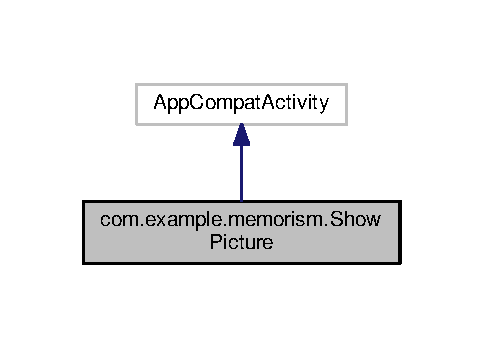
\includegraphics[width=232pt]{de/dc0/classcom_1_1example_1_1memorism_1_1_show_picture__inherit__graph}
\end{center}
\end{figure}


Collaboration diagram for com.\+example.\+memorism.\+Show\+Picture\+:\nopagebreak
\begin{figure}[H]
\begin{center}
\leavevmode
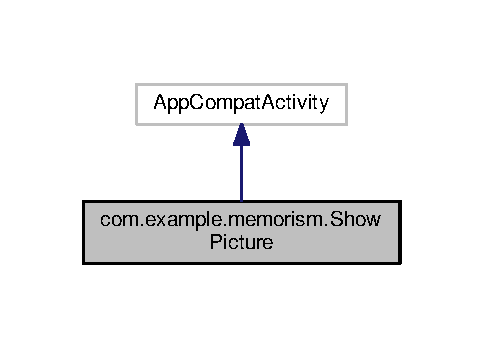
\includegraphics[width=232pt]{d2/d9f/classcom_1_1example_1_1memorism_1_1_show_picture__coll__graph}
\end{center}
\end{figure}
\subsection*{Static Public Member Functions}
\begin{DoxyCompactItemize}
\item 
static Bitmap \hyperlink{classcom_1_1example_1_1memorism_1_1_show_picture_abcf63f664625879f223f6decad593f16}{Rotate\+Bitmap} (Bitmap source, float angle)
\end{DoxyCompactItemize}
\subsection*{Protected Member Functions}
\begin{DoxyCompactItemize}
\item 
void \hyperlink{classcom_1_1example_1_1memorism_1_1_show_picture_a78dce202434c45e590b66c0de64d6b5d}{on\+Create} (Bundle saved\+Instance\+State)
\end{DoxyCompactItemize}


\subsection{Detailed Description}


Definition at line 20 of file Show\+Picture.\+java.



\subsection{Member Function Documentation}
\index{com\+::example\+::memorism\+::\+Show\+Picture@{com\+::example\+::memorism\+::\+Show\+Picture}!on\+Create@{on\+Create}}
\index{on\+Create@{on\+Create}!com\+::example\+::memorism\+::\+Show\+Picture@{com\+::example\+::memorism\+::\+Show\+Picture}}
\subsubsection[{\texorpdfstring{on\+Create(\+Bundle saved\+Instance\+State)}{onCreate(Bundle savedInstanceState)}}]{\setlength{\rightskip}{0pt plus 5cm}void com.\+example.\+memorism.\+Show\+Picture.\+on\+Create (
\begin{DoxyParamCaption}
\item[{Bundle}]{saved\+Instance\+State}
\end{DoxyParamCaption}
)\hspace{0.3cm}{\ttfamily [protected]}}\hypertarget{classcom_1_1example_1_1memorism_1_1_show_picture_a78dce202434c45e590b66c0de64d6b5d}{}\label{classcom_1_1example_1_1memorism_1_1_show_picture_a78dce202434c45e590b66c0de64d6b5d}


Definition at line 23 of file Show\+Picture.\+java.

\index{com\+::example\+::memorism\+::\+Show\+Picture@{com\+::example\+::memorism\+::\+Show\+Picture}!Rotate\+Bitmap@{Rotate\+Bitmap}}
\index{Rotate\+Bitmap@{Rotate\+Bitmap}!com\+::example\+::memorism\+::\+Show\+Picture@{com\+::example\+::memorism\+::\+Show\+Picture}}
\subsubsection[{\texorpdfstring{Rotate\+Bitmap(\+Bitmap source, float angle)}{RotateBitmap(Bitmap source, float angle)}}]{\setlength{\rightskip}{0pt plus 5cm}static Bitmap com.\+example.\+memorism.\+Show\+Picture.\+Rotate\+Bitmap (
\begin{DoxyParamCaption}
\item[{Bitmap}]{source, }
\item[{float}]{angle}
\end{DoxyParamCaption}
)\hspace{0.3cm}{\ttfamily [static]}}\hypertarget{classcom_1_1example_1_1memorism_1_1_show_picture_abcf63f664625879f223f6decad593f16}{}\label{classcom_1_1example_1_1memorism_1_1_show_picture_abcf63f664625879f223f6decad593f16}


Definition at line 46 of file Show\+Picture.\+java.



The documentation for this class was generated from the following file\+:\begin{DoxyCompactItemize}
\item 
/home/farid/\+Android\+Studio\+Projects/\+Memorism/app/src/main/java/com/example/memorism/\hyperlink{_show_picture_8java}{Show\+Picture.\+java}\end{DoxyCompactItemize}

\hypertarget{classcom_1_1example_1_1memorism_1_1take__photo}{}\section{com.\+example.\+memorism.\+take\+\_\+photo Class Reference}
\label{classcom_1_1example_1_1memorism_1_1take__photo}\index{com.\+example.\+memorism.\+take\+\_\+photo@{com.\+example.\+memorism.\+take\+\_\+photo}}


Inheritance diagram for com.\+example.\+memorism.\+take\+\_\+photo\+:\nopagebreak
\begin{figure}[H]
\begin{center}
\leavevmode
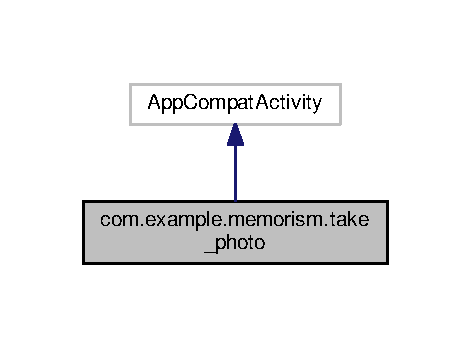
\includegraphics[width=226pt]{d9/d92/classcom_1_1example_1_1memorism_1_1take__photo__inherit__graph}
\end{center}
\end{figure}


Collaboration diagram for com.\+example.\+memorism.\+take\+\_\+photo\+:\nopagebreak
\begin{figure}[H]
\begin{center}
\leavevmode
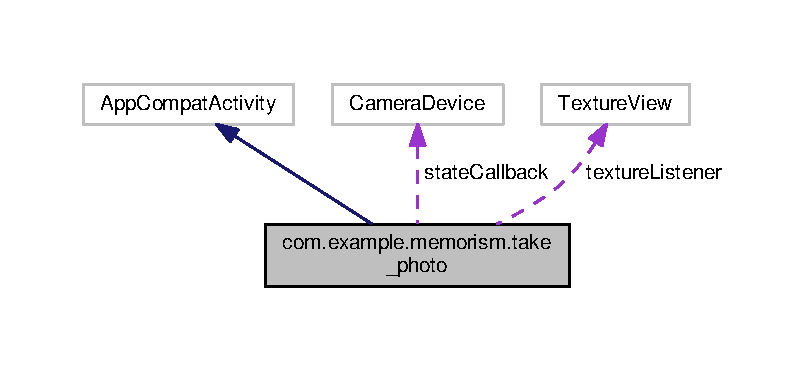
\includegraphics[width=350pt]{dd/d80/classcom_1_1example_1_1memorism_1_1take__photo__coll__graph}
\end{center}
\end{figure}
\subsection*{Public Member Functions}
\begin{DoxyCompactItemize}
\item 
void \hyperlink{classcom_1_1example_1_1memorism_1_1take__photo_a01baf490997362acf99a51951aa61d72}{on\+Request\+Permissions\+Result} (int request\+Code,@Non\+Null String\mbox{[}$\,$\mbox{]} permissions,@Non\+Null int\mbox{[}$\,$\mbox{]} grant\+Results)
\end{DoxyCompactItemize}
\subsection*{Protected Member Functions}
\begin{DoxyCompactItemize}
\item 
void \hyperlink{classcom_1_1example_1_1memorism_1_1take__photo_a9f8e83bcd2e2e8c4543c2c569c5cf011}{on\+Create} (Bundle saved\+Instance\+State)
\item 
void \hyperlink{classcom_1_1example_1_1memorism_1_1take__photo_a557380c5b11f51a683069de65148490c}{on\+Resume} ()
\item 
void \hyperlink{classcom_1_1example_1_1memorism_1_1take__photo_a6005794d6cb9da9347338f9c19f333af}{on\+Pause} ()
\end{DoxyCompactItemize}


\subsection{Detailed Description}


Definition at line 45 of file take\+\_\+photo.\+java.



\subsection{Member Function Documentation}
\index{com\+::example\+::memorism\+::take\+\_\+photo@{com\+::example\+::memorism\+::take\+\_\+photo}!on\+Create@{on\+Create}}
\index{on\+Create@{on\+Create}!com\+::example\+::memorism\+::take\+\_\+photo@{com\+::example\+::memorism\+::take\+\_\+photo}}
\subsubsection[{\texorpdfstring{on\+Create(\+Bundle saved\+Instance\+State)}{onCreate(Bundle savedInstanceState)}}]{\setlength{\rightskip}{0pt plus 5cm}void com.\+example.\+memorism.\+take\+\_\+photo.\+on\+Create (
\begin{DoxyParamCaption}
\item[{Bundle}]{saved\+Instance\+State}
\end{DoxyParamCaption}
)\hspace{0.3cm}{\ttfamily [protected]}}\hypertarget{classcom_1_1example_1_1memorism_1_1take__photo_a9f8e83bcd2e2e8c4543c2c569c5cf011}{}\label{classcom_1_1example_1_1memorism_1_1take__photo_a9f8e83bcd2e2e8c4543c2c569c5cf011}


Definition at line 94 of file take\+\_\+photo.\+java.

\index{com\+::example\+::memorism\+::take\+\_\+photo@{com\+::example\+::memorism\+::take\+\_\+photo}!on\+Pause@{on\+Pause}}
\index{on\+Pause@{on\+Pause}!com\+::example\+::memorism\+::take\+\_\+photo@{com\+::example\+::memorism\+::take\+\_\+photo}}
\subsubsection[{\texorpdfstring{on\+Pause()}{onPause()}}]{\setlength{\rightskip}{0pt plus 5cm}void com.\+example.\+memorism.\+take\+\_\+photo.\+on\+Pause (
\begin{DoxyParamCaption}
{}
\end{DoxyParamCaption}
)\hspace{0.3cm}{\ttfamily [protected]}}\hypertarget{classcom_1_1example_1_1memorism_1_1take__photo_a6005794d6cb9da9347338f9c19f333af}{}\label{classcom_1_1example_1_1memorism_1_1take__photo_a6005794d6cb9da9347338f9c19f333af}


Definition at line 340 of file take\+\_\+photo.\+java.

\index{com\+::example\+::memorism\+::take\+\_\+photo@{com\+::example\+::memorism\+::take\+\_\+photo}!on\+Request\+Permissions\+Result@{on\+Request\+Permissions\+Result}}
\index{on\+Request\+Permissions\+Result@{on\+Request\+Permissions\+Result}!com\+::example\+::memorism\+::take\+\_\+photo@{com\+::example\+::memorism\+::take\+\_\+photo}}
\subsubsection[{\texorpdfstring{on\+Request\+Permissions\+Result(int request\+Code,"@Non\+Null String[] permissions,"@Non\+Null int[] grant\+Results)}{onRequestPermissionsResult(int requestCode,@NonNull String[] permissions,@NonNull int[] grantResults)}}]{\setlength{\rightskip}{0pt plus 5cm}void com.\+example.\+memorism.\+take\+\_\+photo.\+on\+Request\+Permissions\+Result (
\begin{DoxyParamCaption}
\item[{int}]{request\+Code, }
\item[{@Non\+Null String\mbox{[}$\,$\mbox{]}}]{permissions, }
\item[{@Non\+Null int\mbox{[}$\,$\mbox{]}}]{grant\+Results}
\end{DoxyParamCaption}
)}\hypertarget{classcom_1_1example_1_1memorism_1_1take__photo_a01baf490997362acf99a51951aa61d72}{}\label{classcom_1_1example_1_1memorism_1_1take__photo_a01baf490997362acf99a51951aa61d72}


Definition at line 318 of file take\+\_\+photo.\+java.

\index{com\+::example\+::memorism\+::take\+\_\+photo@{com\+::example\+::memorism\+::take\+\_\+photo}!on\+Resume@{on\+Resume}}
\index{on\+Resume@{on\+Resume}!com\+::example\+::memorism\+::take\+\_\+photo@{com\+::example\+::memorism\+::take\+\_\+photo}}
\subsubsection[{\texorpdfstring{on\+Resume()}{onResume()}}]{\setlength{\rightskip}{0pt plus 5cm}void com.\+example.\+memorism.\+take\+\_\+photo.\+on\+Resume (
\begin{DoxyParamCaption}
{}
\end{DoxyParamCaption}
)\hspace{0.3cm}{\ttfamily [protected]}}\hypertarget{classcom_1_1example_1_1memorism_1_1take__photo_a557380c5b11f51a683069de65148490c}{}\label{classcom_1_1example_1_1memorism_1_1take__photo_a557380c5b11f51a683069de65148490c}


Definition at line 330 of file take\+\_\+photo.\+java.



The documentation for this class was generated from the following file\+:\begin{DoxyCompactItemize}
\item 
/home/farid/\+Android\+Studio\+Projects/\+Memorism/app/src/main/java/com/example/memorism/\hyperlink{take__photo_8java}{take\+\_\+photo.\+java}\end{DoxyCompactItemize}

\input{dd/d2b/classcom_1_1example_1_1memorism_1_1_triplist___adaptater_1_1_trip__list_view_holder}
\input{d1/da4/classcom_1_1example_1_1memorism_1_1_triplist___adaptater}
\input{dc/d9e/classcom_1_1example_1_1memorism_1_1_trip_list_activity}
\chapter{File Documentation}
\hypertarget{create__memory_8java}{}\section{/home/farid/\+Android\+Studio\+Projects/\+Memorism/app/src/main/java/com/example/memorism/create\+\_\+memory.java File Reference}
\label{create__memory_8java}\index{/home/farid/\+Android\+Studio\+Projects/\+Memorism/app/src/main/java/com/example/memorism/create\+\_\+memory.\+java@{/home/farid/\+Android\+Studio\+Projects/\+Memorism/app/src/main/java/com/example/memorism/create\+\_\+memory.\+java}}
\subsection*{Classes}
\begin{DoxyCompactItemize}
\item 
class \hyperlink{classcom_1_1example_1_1memorism_1_1create__memory}{com.\+example.\+memorism.\+create\+\_\+memory}
\end{DoxyCompactItemize}
\subsection*{Packages}
\begin{DoxyCompactItemize}
\item 
package \hyperlink{namespacecom_1_1example_1_1memorism}{com.\+example.\+memorism}
\end{DoxyCompactItemize}

\input{de/dc9/create__trip_8java}
\hypertarget{_g_p_stracker_8java}{}\section{/home/farid/\+Android\+Studio\+Projects/\+Memorism/app/src/main/java/com/example/memorism/\+G\+P\+Stracker.java File Reference}
\label{_g_p_stracker_8java}\index{/home/farid/\+Android\+Studio\+Projects/\+Memorism/app/src/main/java/com/example/memorism/\+G\+P\+Stracker.\+java@{/home/farid/\+Android\+Studio\+Projects/\+Memorism/app/src/main/java/com/example/memorism/\+G\+P\+Stracker.\+java}}
\subsection*{Classes}
\begin{DoxyCompactItemize}
\item 
class \hyperlink{classcom_1_1example_1_1memorism_1_1_g_p_stracker}{com.\+example.\+memorism.\+G\+P\+Stracker}
\end{DoxyCompactItemize}
\subsection*{Packages}
\begin{DoxyCompactItemize}
\item 
package \hyperlink{namespacecom_1_1example_1_1memorism}{com.\+example.\+memorism}
\end{DoxyCompactItemize}

\hypertarget{_item_detail_activity_8java}{}\section{/home/farid/\+Android\+Studio\+Projects/\+Memorism/app/src/main/java/com/example/memorism/\+Item\+Detail\+Activity.java File Reference}
\label{_item_detail_activity_8java}\index{/home/farid/\+Android\+Studio\+Projects/\+Memorism/app/src/main/java/com/example/memorism/\+Item\+Detail\+Activity.\+java@{/home/farid/\+Android\+Studio\+Projects/\+Memorism/app/src/main/java/com/example/memorism/\+Item\+Detail\+Activity.\+java}}
\subsection*{Classes}
\begin{DoxyCompactItemize}
\item 
class \hyperlink{classcom_1_1example_1_1memorism_1_1_item_detail_activity}{com.\+example.\+memorism.\+Item\+Detail\+Activity}
\end{DoxyCompactItemize}
\subsection*{Packages}
\begin{DoxyCompactItemize}
\item 
package \hyperlink{namespacecom_1_1example_1_1memorism}{com.\+example.\+memorism}
\end{DoxyCompactItemize}

\hypertarget{_item_detail_fragment_8java}{}\section{/home/farid/\+Android\+Studio\+Projects/\+Memorism/app/src/main/java/com/example/memorism/\+Item\+Detail\+Fragment.java File Reference}
\label{_item_detail_fragment_8java}\index{/home/farid/\+Android\+Studio\+Projects/\+Memorism/app/src/main/java/com/example/memorism/\+Item\+Detail\+Fragment.\+java@{/home/farid/\+Android\+Studio\+Projects/\+Memorism/app/src/main/java/com/example/memorism/\+Item\+Detail\+Fragment.\+java}}
\subsection*{Classes}
\begin{DoxyCompactItemize}
\item 
class \hyperlink{classcom_1_1example_1_1memorism_1_1_item_detail_fragment}{com.\+example.\+memorism.\+Item\+Detail\+Fragment}
\end{DoxyCompactItemize}
\subsection*{Packages}
\begin{DoxyCompactItemize}
\item 
package \hyperlink{namespacecom_1_1example_1_1memorism}{com.\+example.\+memorism}
\end{DoxyCompactItemize}

\hypertarget{_item_list_activity_8java}{}\section{/home/farid/\+Android\+Studio\+Projects/\+Memorism/app/src/main/java/com/example/memorism/\+Item\+List\+Activity.java File Reference}
\label{_item_list_activity_8java}\index{/home/farid/\+Android\+Studio\+Projects/\+Memorism/app/src/main/java/com/example/memorism/\+Item\+List\+Activity.\+java@{/home/farid/\+Android\+Studio\+Projects/\+Memorism/app/src/main/java/com/example/memorism/\+Item\+List\+Activity.\+java}}
\subsection*{Classes}
\begin{DoxyCompactItemize}
\item 
class \hyperlink{classcom_1_1example_1_1memorism_1_1_item_list_activity}{com.\+example.\+memorism.\+Item\+List\+Activity}
\item 
class {\bfseries com.\+example.\+memorism.\+Item\+List\+Activity.\+Simple\+Item\+Recycler\+View\+Adapter}
\item 
class {\bfseries com.\+example.\+memorism.\+Item\+List\+Activity.\+Simple\+Item\+Recycler\+View\+Adapter.\+View\+Holder}
\end{DoxyCompactItemize}
\subsection*{Packages}
\begin{DoxyCompactItemize}
\item 
package \hyperlink{namespacecom_1_1example_1_1memorism}{com.\+example.\+memorism}
\end{DoxyCompactItemize}

\hypertarget{_main_menu_8java}{}\section{/home/farid/\+Android\+Studio\+Projects/\+Memorism/app/src/main/java/com/example/memorism/\+Main\+Menu.java File Reference}
\label{_main_menu_8java}\index{/home/farid/\+Android\+Studio\+Projects/\+Memorism/app/src/main/java/com/example/memorism/\+Main\+Menu.\+java@{/home/farid/\+Android\+Studio\+Projects/\+Memorism/app/src/main/java/com/example/memorism/\+Main\+Menu.\+java}}
\subsection*{Classes}
\begin{DoxyCompactItemize}
\item 
class \hyperlink{classcom_1_1example_1_1memorism_1_1_main_menu}{com.\+example.\+memorism.\+Main\+Menu}
\end{DoxyCompactItemize}
\subsection*{Packages}
\begin{DoxyCompactItemize}
\item 
package \hyperlink{namespacecom_1_1example_1_1memorism}{com.\+example.\+memorism}
\end{DoxyCompactItemize}

\hypertarget{_d_b_helper_8java}{}\section{/home/farid/\+Android\+Studio\+Projects/\+Memorism/app/src/main/java/com/example/memorism/memory/\+D\+B\+Helper.java File Reference}
\label{_d_b_helper_8java}\index{/home/farid/\+Android\+Studio\+Projects/\+Memorism/app/src/main/java/com/example/memorism/memory/\+D\+B\+Helper.\+java@{/home/farid/\+Android\+Studio\+Projects/\+Memorism/app/src/main/java/com/example/memorism/memory/\+D\+B\+Helper.\+java}}
\subsection*{Classes}
\begin{DoxyCompactItemize}
\item 
class \hyperlink{classcom_1_1example_1_1memorism_1_1memory_1_1_d_b_helper}{com.\+example.\+memorism.\+memory.\+D\+B\+Helper}
\begin{DoxyCompactList}\small\item\em this class provide method allowing interaction with the database \end{DoxyCompactList}\end{DoxyCompactItemize}
\subsection*{Packages}
\begin{DoxyCompactItemize}
\item 
package \hyperlink{namespacecom_1_1example_1_1memorism_1_1memory}{com.\+example.\+memorism.\+memory}
\end{DoxyCompactItemize}

\hypertarget{_memory_content_8java}{}\section{/home/farid/\+Android\+Studio\+Projects/\+Memorism/app/src/main/java/com/example/memorism/memory/\+Memory\+Content.java File Reference}
\label{_memory_content_8java}\index{/home/farid/\+Android\+Studio\+Projects/\+Memorism/app/src/main/java/com/example/memorism/memory/\+Memory\+Content.\+java@{/home/farid/\+Android\+Studio\+Projects/\+Memorism/app/src/main/java/com/example/memorism/memory/\+Memory\+Content.\+java}}
\subsection*{Classes}
\begin{DoxyCompactItemize}
\item 
class \hyperlink{classcom_1_1example_1_1memorism_1_1memory_1_1_memory_content}{com.\+example.\+memorism.\+memory.\+Memory\+Content}
\item 
class {\bfseries com.\+example.\+memorism.\+memory.\+Memory\+Content.\+Memory\+Item}
\end{DoxyCompactItemize}
\subsection*{Packages}
\begin{DoxyCompactItemize}
\item 
package \hyperlink{namespacecom_1_1example_1_1memorism_1_1memory}{com.\+example.\+memorism.\+memory}
\end{DoxyCompactItemize}

\hypertarget{misc__funct_8java}{}\section{/home/farid/\+Android\+Studio\+Projects/\+Memorism/app/src/main/java/com/example/memorism/misc\+\_\+funct.java File Reference}
\label{misc__funct_8java}\index{/home/farid/\+Android\+Studio\+Projects/\+Memorism/app/src/main/java/com/example/memorism/misc\+\_\+funct.\+java@{/home/farid/\+Android\+Studio\+Projects/\+Memorism/app/src/main/java/com/example/memorism/misc\+\_\+funct.\+java}}
\subsection*{Classes}
\begin{DoxyCompactItemize}
\item 
class \hyperlink{classcom_1_1example_1_1memorism_1_1misc__funct}{com.\+example.\+memorism.\+misc\+\_\+funct}
\end{DoxyCompactItemize}
\subsection*{Packages}
\begin{DoxyCompactItemize}
\item 
package \hyperlink{namespacecom_1_1example_1_1memorism}{com.\+example.\+memorism}
\end{DoxyCompactItemize}

\hypertarget{_show___map_8java}{}\section{/home/farid/\+Android\+Studio\+Projects/\+Memorism/app/src/main/java/com/example/memorism/\+Show\+\_\+\+Map.java File Reference}
\label{_show___map_8java}\index{/home/farid/\+Android\+Studio\+Projects/\+Memorism/app/src/main/java/com/example/memorism/\+Show\+\_\+\+Map.\+java@{/home/farid/\+Android\+Studio\+Projects/\+Memorism/app/src/main/java/com/example/memorism/\+Show\+\_\+\+Map.\+java}}
\subsection*{Classes}
\begin{DoxyCompactItemize}
\item 
class \hyperlink{classcom_1_1example_1_1memorism_1_1_show___map}{com.\+example.\+memorism.\+Show\+\_\+\+Map}
\end{DoxyCompactItemize}
\subsection*{Packages}
\begin{DoxyCompactItemize}
\item 
package \hyperlink{namespacecom_1_1example_1_1memorism}{com.\+example.\+memorism}
\end{DoxyCompactItemize}

\hypertarget{_show_picture_8java}{}\section{/home/farid/\+Android\+Studio\+Projects/\+Memorism/app/src/main/java/com/example/memorism/\+Show\+Picture.java File Reference}
\label{_show_picture_8java}\index{/home/farid/\+Android\+Studio\+Projects/\+Memorism/app/src/main/java/com/example/memorism/\+Show\+Picture.\+java@{/home/farid/\+Android\+Studio\+Projects/\+Memorism/app/src/main/java/com/example/memorism/\+Show\+Picture.\+java}}
\subsection*{Classes}
\begin{DoxyCompactItemize}
\item 
class \hyperlink{classcom_1_1example_1_1memorism_1_1_show_picture}{com.\+example.\+memorism.\+Show\+Picture}
\end{DoxyCompactItemize}
\subsection*{Packages}
\begin{DoxyCompactItemize}
\item 
package \hyperlink{namespacecom_1_1example_1_1memorism}{com.\+example.\+memorism}
\end{DoxyCompactItemize}

\hypertarget{take__photo_8java}{}\section{/home/farid/\+Android\+Studio\+Projects/\+Memorism/app/src/main/java/com/example/memorism/take\+\_\+photo.java File Reference}
\label{take__photo_8java}\index{/home/farid/\+Android\+Studio\+Projects/\+Memorism/app/src/main/java/com/example/memorism/take\+\_\+photo.\+java@{/home/farid/\+Android\+Studio\+Projects/\+Memorism/app/src/main/java/com/example/memorism/take\+\_\+photo.\+java}}
\subsection*{Classes}
\begin{DoxyCompactItemize}
\item 
class \hyperlink{classcom_1_1example_1_1memorism_1_1take__photo}{com.\+example.\+memorism.\+take\+\_\+photo}
\end{DoxyCompactItemize}
\subsection*{Packages}
\begin{DoxyCompactItemize}
\item 
package \hyperlink{namespacecom_1_1example_1_1memorism}{com.\+example.\+memorism}
\end{DoxyCompactItemize}

\input{d3/d83/_triplist___adaptater_8java}
\input{de/d9d/_trip_list_activity_8java}
%--- End generated contents ---

% Index
\backmatter
\newpage
\phantomsection
\clearemptydoublepage
\addcontentsline{toc}{chapter}{Index}
\printindex

\end{document}
